% Szkielet pracy:
%
% Copyright (c) 2001 by Marcin Woliñski <M.Wolinski@gust.org.pl>
% Poprawki spowodowane zmianami przepisów - Marcin Szczuka, 1.10.2004
% Poprawki spowodowane zmianami przepisow i ujednolicenie 
% - Seweryn Kar³owicz, 05.05.2006
% dodaj opcjê [licencjacka] dla pracy licencjackiej
%

\documentclass[licencjacka]{pracamgr}

\usepackage{polski}
\usepackage[utf8]{inputenc}
\usepackage{verbatim}
\usepackage{color}
\usepackage{hyperref}
\usepackage{graphicx}

% Tutaj każdy wstawia swoje dane drukując pracę licencjacką
\author{Krzysztof Gogolewski, Karol Nienałtowski\\Jakub Oćwieja, Michał Sabaciński}
\nralbumu{291538, 292692, 292690, 292511}

\title{Pengurus - system zarządzania biurem tłumaczeń}

\tytulang{Pengurus - translation agency management system}

\kierunek{Informatyka}

% Praca wykonana pod kierunkiem:
% (poda¿ tytu¿/stopie¿ imi¿ i nazwisko opiekuna
% Instytut
% ew. Wydzia¿ ew. Uczelnia (je¿eli nie MIM UW))
\opiekun{Michał Możdżonek}

\date{Czerwiec 2012}

%Dziedzina wg klasyfikacji Socrates-Erasmus:
\dziedzina{ 
11.3 Informatyka\\ 
}

%Klasyfikacja tematyczna wedlug AMS (matematyka) lub ACM (informatyka)
\klasyfikacja{D. Software\\
  D.2. Software engineering\\
  D.2.9 Management}

% S¿owa kluczowe:
\keywords{system, zarządzanie, tłumacz, tłumaczenie, aplikacja, firma, biuro}

% Miejsce na w¿asne makra i ¿rodowiska:
\newtheorem{defi}{Definicja}[section]

% koniec definicji

\begin{document}
\maketitle

%tu idzie streszczenie na strone poczatkowa
\begin{abstract}
  W pracy przedstawiono przebieg projektowania i implementacji projektu Pengurus, czyli systemu do zarządzania biurem tłumaczeń.
  W kolejnych rozdziałach opisane zostały: nasz projekt, odniesienie do konkurencyjnych produktów, wyniki pracy, użyte narzędzia i technologie oraz sam przebieg wykonania projektu.
\end{abstract}

\tableofcontents
%\listoffigures
%\listoftables

\chapter{Wprowadzenie - Wizja}
\section{Miejsce na rynku}
W dzisiejszym świecie bardzo istotną kwestią wydaje się być szeroko pojęte usprawnianie zarządzania firmą. 
Jednym z najważniejszych jego aspektów jest przyspieszanie i formalizacja przebiegu procesu biznesowego. 
Problem ten można rozwiązać, dokonując jego informatyzacji przy użyciu najnowszych technologii dostępnych na rynku, co okazuje się być jednym z najłatwiejszych i najtańszych rozwiązań. \\

Z podobnym problemem muszą zmierzyć się również biura tłumaczeń. Duża konkurencja wymaga od nich: 
\begin{itemize}
\item usprawniania procesu tłumaczenia, 
\item ułatwienia kontaktu na linii biuro - klient, 
\item ułatwienia kontaktu na linii biuro - pracownicy nieetatowi (pracujący zazwyczaj poza siedzibą firmy), 
\item możliwości wprowadzenia szybkich korekt,
\item wysokiego bezpieczeństwa przechowywania danych (dane osobowe, pliki, własność intelektualna),
\item prostoty użytkowania,
\item powszechnego dostępu. 
\end{itemize} 

Oczywiście na rynku znajdują się produkty, które są przeznaczone do zarządzania biurem tłumaczeń, 
są one jednak ograniczone jedynie do pracowników biura (nie jest możliwa praca mobilna),
bądź w przypadku aplikacji webowych zostały stworzone przy użyciu starych technologii (np. PHP). 
Ponadto produkty te często zapewniają niski poziom bezpieczeństwa i nie są przeznaczone do kontaktów z klientami.
Pengurus CRM ma być aplikacją, która wychodzi naprzeciw tym problemom. 
Będzie to pierwsza na rynku aplikacja WWW stworzona przy użyciu gamy nowych technnologii - ExtGWT, Hibernate, Spring.
Skierowana bezpośrednio do właścicieli biur tłumaczeń, w znacznym stopniu ułatwiająca kontakt z klientem, jak również kontakt pomiędzy pracownikami. 
Do jej obsługi będzie wystarczać przeglądarka WWW, zatem umożliwi to pracę poza biurem
oraz skróci klientowi czas jaki musi poświęcić na nadzorowanie projektu. 

\section{Użytkownicy}
\begin{itemize}
\item Kierownik (ang. Executive) – pracownik firmy, posiadający najwięcej praw w systemie Pengurus, fizycznie rola przewidziana dla osób postawionych najwyżej w hierarchii firmy. Jako jedyny posiada dostęp do panelu administratora.
\item Menadżer Projektu (ang. Project Manager)– pracownik firmy, odpowiadający za nadzorowanie projektów.
\item Ekspert (ang. Expert)– pracownik firmy, odpowiedzialny za tłumaczenie dokumentów, zleconych przez Menadżera Projektu (Tłumacz).
\item Księgowy (ang. Accountant)– pracownik firmy, odpowiedzialny za księgowość firmy.
\item Pracownik nieetatowy (ang. Freelancer)– osoba nie będąca na stałe zatrudniona w firmie, która na potrzeby chwili wykonuje odpłatnie zlecone tłumaczenia (Tłumacz).
\item Klient (ang. Client)– klient indywidualny bądź biznesowy zlecający tłumaczenie firmie.
\end{itemize}

\section{Przypadki użycia}
\begin{itemize} 
\item Przyjęcie zlecenia

Kierownik zlecenia ( Menadżer ds. produkcji/ Stanowisko ds. relacji z klientami i produkcji ) 
jest odpowiedzialny za przyjęcie zlecenia od klienta oraz przygotowanie odpowiedniej oferty, 
która następnie zostaje podana ocenie klientowi.

Kierownik zlecenia odbiera dokumenty od klienta wraz z tekstem oryginału , zapoznaje się on z przesłanym/odebranym materiałem,
a następnie ustala ze zlecającym szczegóły dotyczące zlecenia takie jak data realizacji, cena,  tryb zlecenia, rodzajem tłumaczenia,  
materiały pomocnicze.

Kierownik zlecenia przgotowuje dziennik zlecenia. W dzienniku zapisywana jest historia pracy z dokumentem i 
odnotowywane są wszystkie istotne zdarzenia mające wpływ na jakość i/lub bezpieczeństwo informacji przekazanych przez klienta. 
Ponadto przechowywane są : data utworzenia zlecenia, data przyjęcia tekstu źródłowego oraz związanych z nim materiałów,
,numer zlecenia, informację o podjętych działaniach w celu usunięcia niezgodności. 

Przed rozpoczęciem realizacji projektu klient jest zobowiązany do zaakceptowania przygotowanej oferty.

\item Rejestracja zlecenia \\
Kierownik zlecenia wyznacza lidera/liderów dla tłumaczenia (Menadżera Projektu). W uzasadnionych przypadkach działania Lidera wykonuje kierownik zlecenia.
Ponadto jest on odpowiedzialny za przypisanie odpowiednich tłumaczy/ weryfikatorów do projektu
Kierownik ponadto udostępnia menadżerom przesłane przez klienta zasoby ( pliki ) i wyznacza im temin realizacji poszczygólnych etapów projektu.

\item Tłumaczenie i weryfikacja\\
Menadżer Projektu przekazuje odpowiednim tłumaczom materiały oraz wyznacza termin realizacji tłumaczenia.
W tym celu tworzy nowe pliki i udostępnia je tłumaczowi.
Ponadto menadżer wyznacza odpwiedniego Weryfikatora.
Tłumacz przesyła pliki ze zrealizownym etapami pracy. Każdy z tych plików może być edytowany przez autora, a dostęp do nich posiadają menadżerowie oraz weryfikatorzy.
Po zakończonym tłumaczeniu weryfikator sprawdza wykonaną pracę, a następnie wysyła plik z poprawkami zapisuje uwagi oraz akceptuje wykonaną pracę lub nakazuje ponowne rozpatrzenie.
Po ostatecznym zaakceptowaniu przez weryfikator menadżer odbiera pliki.
W przypadku pracowników nieetatowych następuje rozliczenie z tłumaczem, które jest potwierdzane przez księgowego.

\item Przekazanie gotowego tłumaczenia do zleceniodawcy\\
Menadżer projektu odbiera od tłumaczy i weryfikatorów pliki oraz przygotowuje ostateczny dokument, który następnie zostaje podany ocenie kierownikowi zlecenia.
Kieronik zlecenia po zaakceptowaniu przekazuje go klientowi, który podaje go swojej ocenie. W razie reklamacji dokument wraz z uwagami zostaje przesłany 
menadżerowi projektu do ponownego rozpatrzenia.

\item Archiwizacja zleceń\\
Po zamknięciu obsługi zlecenia – formularz zlecenia przechowywany jest,
wraz z adnotacją dotyczącą danych faktury oraz danych określających uczestników 
procesu realizacji, w wersji papierowej w kolejności odpowiadającej numerom 
wewnętrznym nadanym na początku procesu.
Pliki danego zlecenia wraz z dziennikiem zlecenia, przechowywane są w 
katalogu przeznaczonym do obsługi danego zlecenia na serwerze.
Dane znajdujące się na serwerze poddawane są archiwizacji, zgodnie z 
Polityką tworzenia kopii zapasowych Pl-4.1

\item Tworzenie i edycja użytkowników systemu\\
Kierownik tworzy użytkownika oraz nadaje mu odpowiednie role ( tłumacz , klient, menadżer projektu, itd. ).
Pracownik posiada : login, dane osobowe i kontaktowe , posiadane umiejętności tłumaczenia ( razem z posiadanymi prawamy - tłumaczenia sądowe, techniczne ).
Klient może być kilentem biznesowym ( posiada pośredników ) , bądź klientem indywidualnym.

\end{itemize}

\chapter{Aplikacja}

\section{Definicje}
\begin{itemize}
\item Oferta (ang. Quote) – przygotowana przez firmę, przedstawiana klientowi, który zgadza się na przedstawione warunki, bądź je renegocjuje. (oferta jest modyfikowana przez firmę). Każda Oferta składa się z Prac i opisu.
\item Praca (ang.Job) – jednostka określająca część zlecenia (np. przetłumaczenie jednego tomu książki), na którą składa się lista Zadań.
\item Projekt (ang.Project)– tworzony jest na podstawie ostatecznej wersji Oferty zaakceptowanej przez dwie strony (klient, firma). Zawiera Prace składające się na Ofertę. Do każdego Projektu przypisany jest co najmniej jeden Menadżer Projektu oraz ewentualnie lista Tłumaczy i Weryfikatorów. Z Prac powstają Zadania.
\item Zadanie (ang. Task) – przypisywane Tłumaczowi i Weryfikatorowi. Każde Zadanie jest częścią dokładnie jednej Pracy.
\end{itemize}
\section{Opis aplikacji}
System Zarządzania Biurem Tłumaczeń Pengurus jest aplikacją przeznczaną dla użytkowników pełniących różne role w procesie tłumaczenia.
Główna strona aplikacji jest podzielona na 3 moduły:
\begin{itemize}
\item Panel górny, w którym użytkownik może wybrać preferowany język, wylogować się oraz zmienić ustawienia
\item  Menu boczne, w którym znajdują się odnośniki do poszczególnych projektów / zadań oraz paneli administracyjnych
\item  Panel główny, w którym wyświetlane są akcje proawdzone przez użytkownika.  
\begin{figure}[h!]
\centering
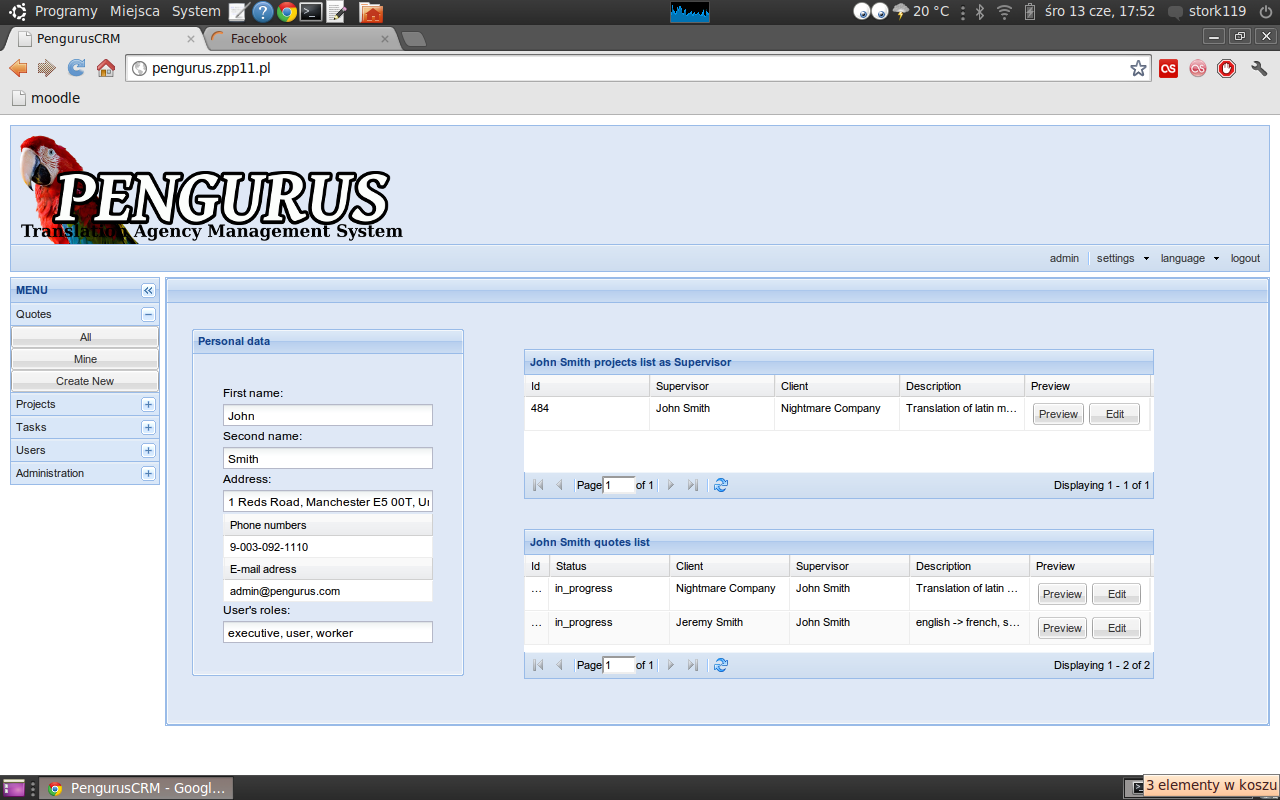
\includegraphics[width=0.8\textwidth]{resources/panel_glowny.png}
\caption{Panel Główny podzielony na 3 moduły}
\end{figure}
\end{itemize}

Zgodnie z założeniami i przypadkami użycia wyróżniliśmy kilka ról użytkowników. W zależności od pełnionej roli użytkownik aplikacji posiada specyficzną bazę uprawnień do zarządzania danymi. W szczególności niektórzy użytkownicy mają zablokowaną możliwość podglądu, bądź edycji niektórych danych. Wszystkie dozwolone operacje - dane do których istnieje dostęp mają odnośnik w menu bocznym.
Więcej szczegółów dotyczących realizacji autoryzacji danych znajduje się w dalszej części pracy.\\

Każdy z użytkowników systemu ma możliwość edytować dane dotyczące jego osoby.\\ 

\begin{figure}[h!]
\centering
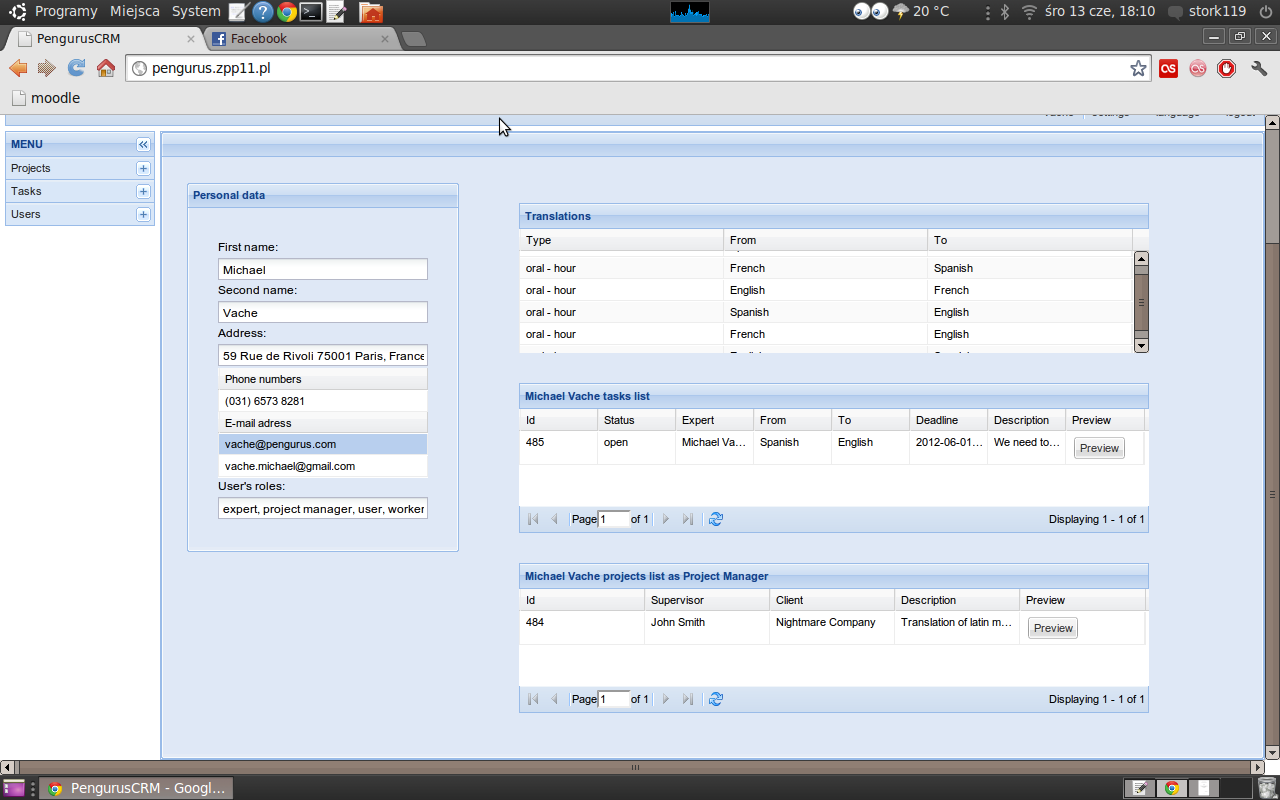
\includegraphics[width=0.8\textwidth]{resources/edycja_danych.png}
\caption{Panel do edycji danych osobowych użytkownika}
\end{figure}

Ponadto każdy Kierownik ma prawo do wglądu i edycji danych osobowych każdego z użykowników. 
Kierownicy będący jednnocześnie administratorami systemu zarządzają aspektami technicznymi.\\
Panel administracyjny udostępnia im między innymi:
\begin{itemize}
\item Zarządzanie użytkownikami - tworzenie, edycja danych osobowych oraz danych zawodowych (np. znajomość języków),
\item  Administrowanie językami - edytowanie oferty dostępnej przez biuro tłumaczeń, dodawnie i edycja języków oraz dostępnych typów tłumaczeń (np. tłumaczenia sądowe, naukowe - informatyczne), przypisywanie stałych cen za jednostkę pracy,
\item  Zarządzanie dodatkowymi danymi - tworzenie bądź usuwanie dostępnej formy płatności.
\begin{figure}[h!]
\centering
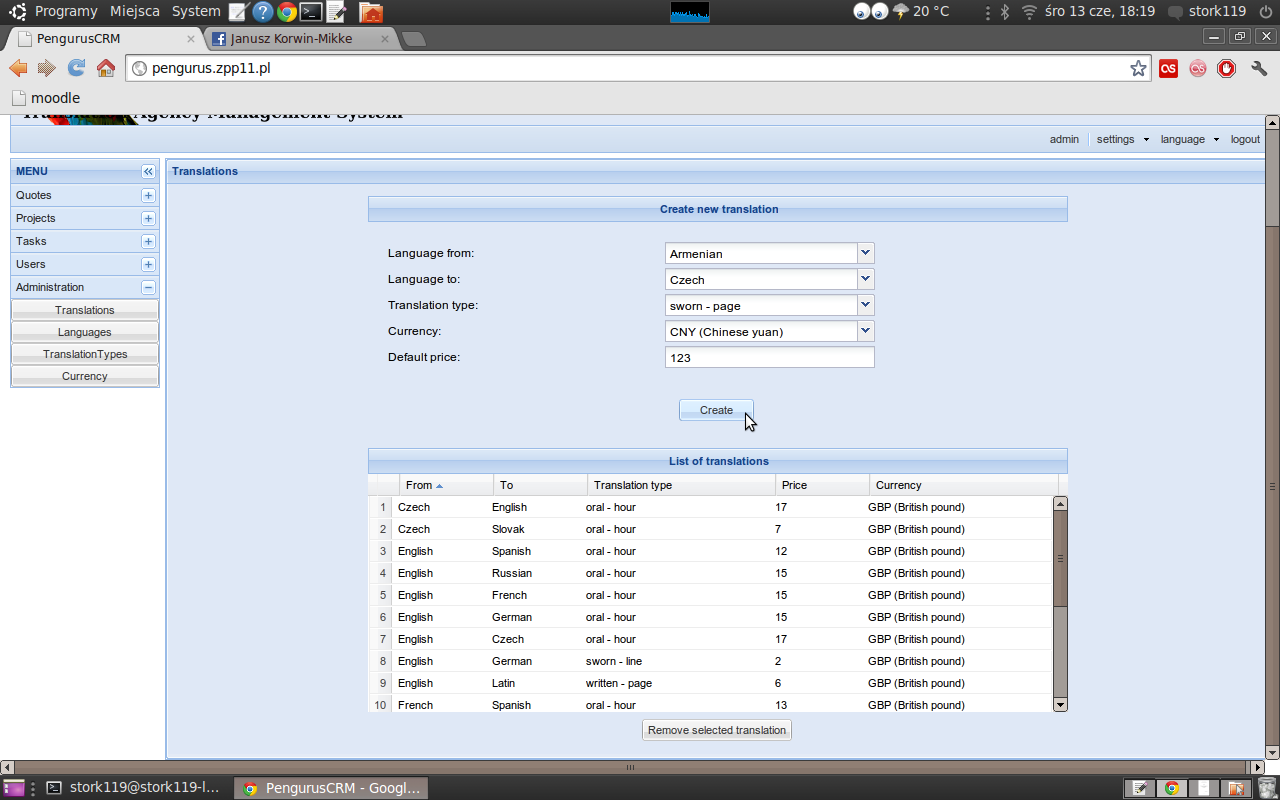
\includegraphics[width=0.7\textwidth]{resources/panel_administracyjny.png}
\caption{Panel Administracyjny - dodanie nowego tłumaczenia}
\end{figure}
\end{itemize}
W celu przedstawienia możliwości, jakie udostępnia aplikacja przedstawimy podstawowy przebieg procesu tłumaczenia od przyjęcia zlecenia od Klienta do ostatecznego przyjęcia rozwiązania.\\
\begin{itemize}
\item Oferta - Jest to pierwszy etap realizacji projektu. Wgląd w niego mają kierownicy, a w szczególności kierownik danej oferty, a także klient.
Przygotowanie Oferty polega na przesłaniu przez klienta odpowiednich plików i dokumentów oraz sprecyzowaniu problemu w opisie.

\begin{figure}[h!]
\centering
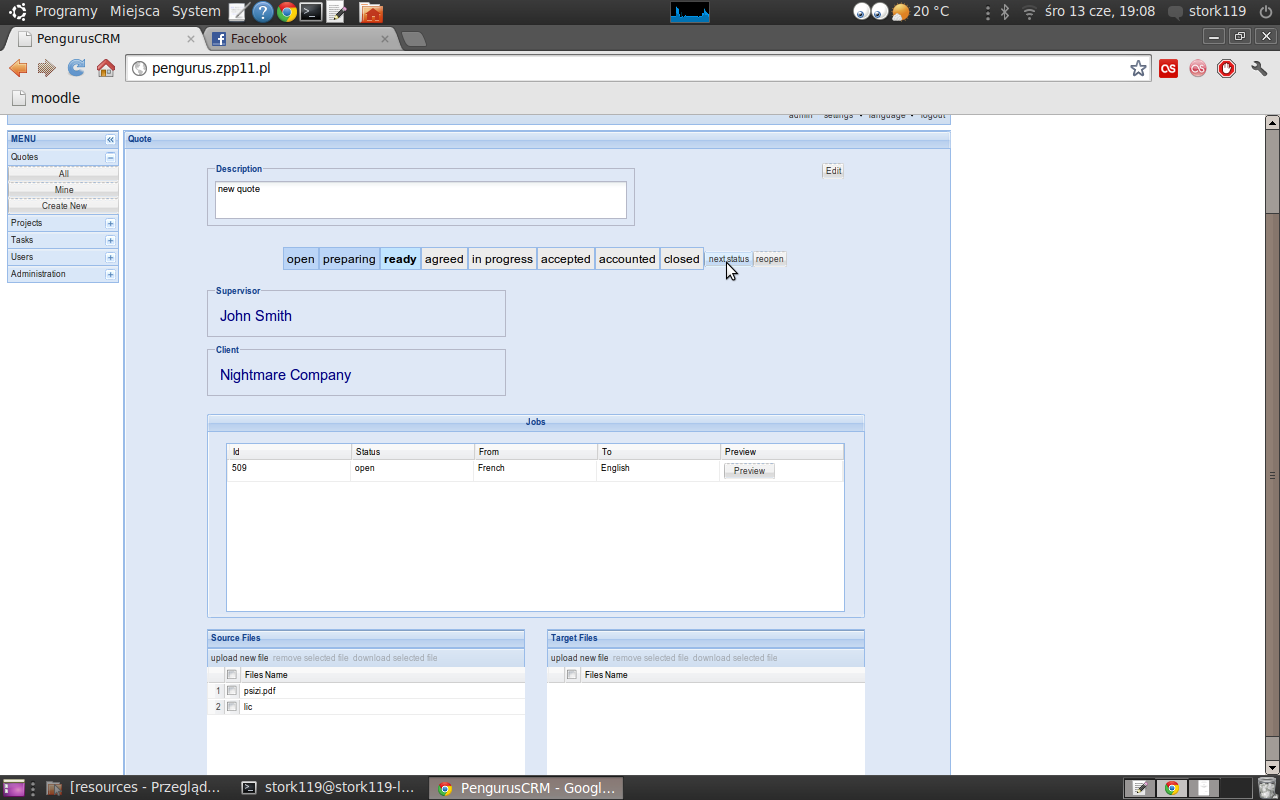
\includegraphics[width=0.8\textwidth]{resources/quote.png}
\caption{Oferta}
\end{figure}

Następnie kierownik oferty jest zobowiązany do podzielenia pracy na poszczególne etapy. W tym celu tworzy Prace, które zawierają:
przydzielone pliki, opis, termin zakończenia pracy,cenę.

\begin{figure}[h!]
\centering
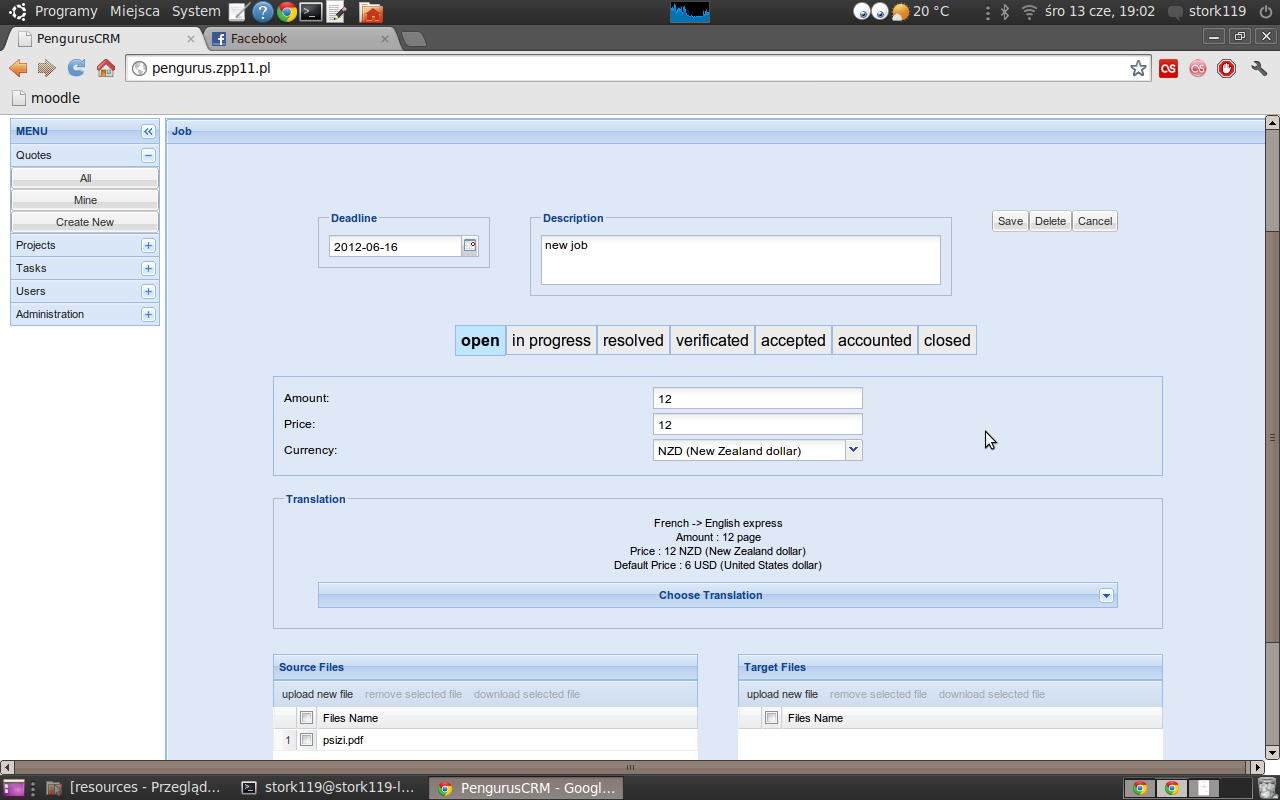
\includegraphics[width=0.8\textwidth]{resources/job.png}
\caption{Stworzona przez Kierownika Praca}
\end{figure}

Tak przygotowana Oferta zostaje poddana ocenie Klienta, który w razie braku uwag akceptuje ją za pomocą odpowiedniego pasku stanu.

\item Projekt - Jest to kolejny etap realizacji zlecenia związany stricte z procesem tłumaczenia. Wgląd w proces tłumaczenia mają Kierownicy oraz Menadżerowie Projektu ,Tłumacze i Weryfikatorzy, którzy zostali wybrani przez kierownika projektu z puli pracowników o odpowiednich do danego Projektu wymogach.\\
\begin{figure}[h!]
\centering
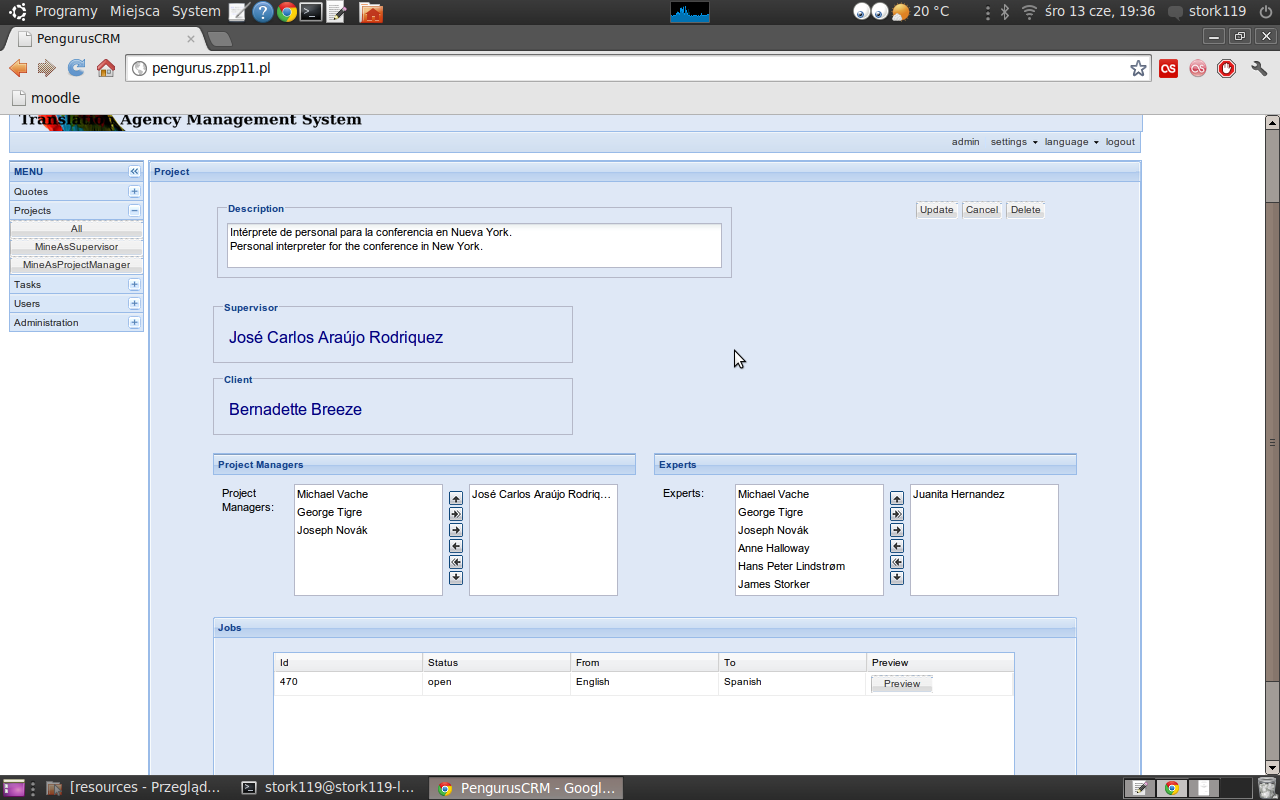
\includegraphics[width=0.8\textwidth]{resources/project.png}
\caption{Projekt - etap realizacji zamówienia}
\end{figure}
 
Menadżerowie Projektów zgodnie z ustalonym podziałem pracy są zobowiązani do podzielenia kolejnych Prac na Zadania, które zlecają Tłumaczom i Weryfikatorom. Są oni odpowiedzialni za ustalenie terminu przyjęcia rozwiązania, przydzielenie odpowiedniego pliku do tłumaczenia oraz ostatecznej oceny pracy zarówno tłumacza, jak i weryfikatora. Szczegółowy opis etapu tłumaczenia (Zadania) zostanie opisany w dalszej części.\\
Po zakończeniu pojedynczej Pracy, tzn. przetłumaczeniu całego tekstu załączonego do Pracy, Menadżerowie Projektu są zobowiązani do przygotowania ostateczenej wersji pliku i udostępnienie jej Klientowi. Klient może za pomocą pasku stanu zaakceptować tak wykonaną Pracę, bądź może poprosić o dokonanie odpowiednich poprawek.

\item Zakończenie  realizacji Pracy - Klient akceptując wykonanie Pracy jest zobowiązany do rozliczenia jej. Gdy takowe nastąpi księgowy zaznacza ten fakt i możliwe jest zakończenie przez Kierownika przebiegu Pracy. 
\item Zakończenie  realizacji Oferty - Gdy zostaną zakończone wszystkie Prace następuje rozliczenie i ostateczne zamknięcie całej Oferty. Zamknięta Oferta wraz ze wszystkimi dokumentami trafia następnie do archiwum. 
\end{itemize}  

\section{Podstawowy przypadek użycia}
Uznaliśmy, że najważniejszym przypadkiem użycia wymagającym głębszego wyjaśnienia jest etap tłumaczenia - Zadanie. Przedstaiwony zostanie on bardziej szczegółowo, aby wyjaśnić wszelkie wątpliwości i ukazać możliwości naszej aplikacji.

\begin{enumerate}
\item	Tworzenie Zadania - Menadżer Projektu odpowiedzialny za daną Pracę tworzy nowe Zadanie wybierając termin, jego realizacji, cenę i walutę w jakiej zostanie rozliczone zadanie oraz opis wyjaśniający problem . Ponadto Menadżer wybiera Tłumacza i Weryfikatora z listy pracowników przydzielonych do Projektu, którzy odpowiadają profilowi danego problemu. \\
\begin{figure}[h!]
\centering
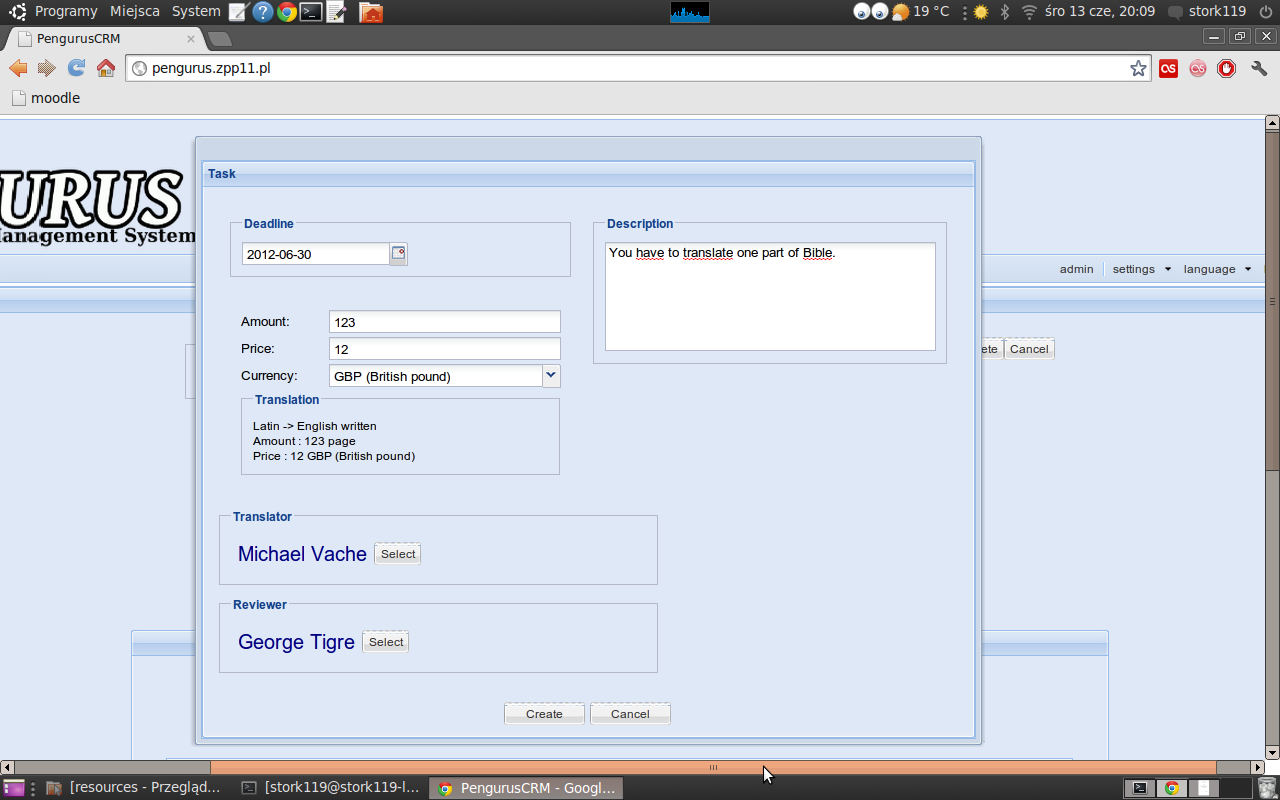
\includegraphics[width=0.8\textwidth]{resources/task_create.png}
\caption{Tworzenie Zadania}
\end{figure}
Po stworzeniu Zadania Menadżer Projektu przydziela pliki, które mają zostać przetłumaczone. Pliki do tłumaczenia są umieszczane w katalogu "Pliki Źródłowe" (ang. Source Files).
\item 	Realizacja Tłumaczenia - Przydzielony do tłumaczenia ekspert przystępuje do jego realizacji zaznaczając to na pasku stanu i przechodząc do etapu "in progress". Ekspert wykonujac swoje zadanie może (a nawet powinien w celu zachowania bezpieczeństwa) po każdym etapie swojej pracy umieścić pliki z cząstkowym rozwiązaniem. Takie pliki powinny się znaleźć w katalogu "Pliki Docelowe" (ang. Target Files).\\
Tłumacz informuje o zakończeniu pracy poprzez umieszczenie rozwiązania w katalogu "Pliki Docelowe" i przejściu na pasku stanu do etapu "resolved".   
\item Weryfikacja - Po rozwiązaniu Zadania następuje etap weryfikacji dokonywany przez przydzieloną do tego osobę. Weryfikator ma za zadanie pobrać odpowiedni plik, a następnie poprawić. W razie poważniejszych błędów weryfikator może umieścić odpowiedni komentarz pod zadaniem i nie przyjąć rozwiązania. Zaznacza to wybierając akcję "re-open" na pasku stanu.	
\begin{figure}[h!]
\centering
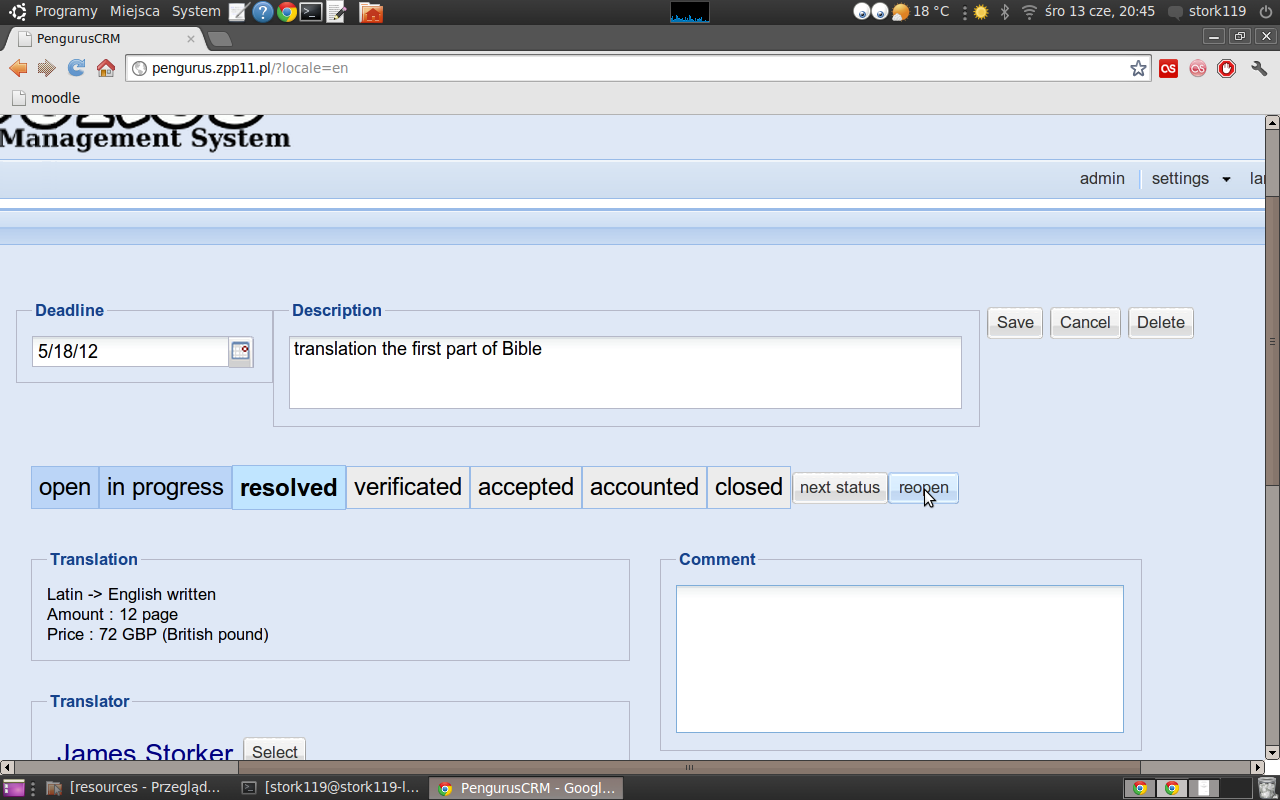
\includegraphics[width=0.8\textwidth]{resources/task_reopen.png}
\caption{Weryfikowanie Zadania - weryfikator nie akceptuje rozwiązania}
\end{figure}
\item 	Przyjęcie rozwiązania przez Menadżera Projektu - Każde Zadanie po zweryfikowniu musi zostać zaakceptowane przez jednego z Menadżerów Projektu. W razie uwag (podobnie jak to było w etapie weryfikacji) Menadżer może ponownie odesłać Zadanie do weryfikatora. Jeśli natomiast nie wymaga ono poprawek zostaje to zaakceptowane, a następnie dołączone do reszty rozwiązania zawartego w Pracy.
\begin{figure}[h!]
\centering
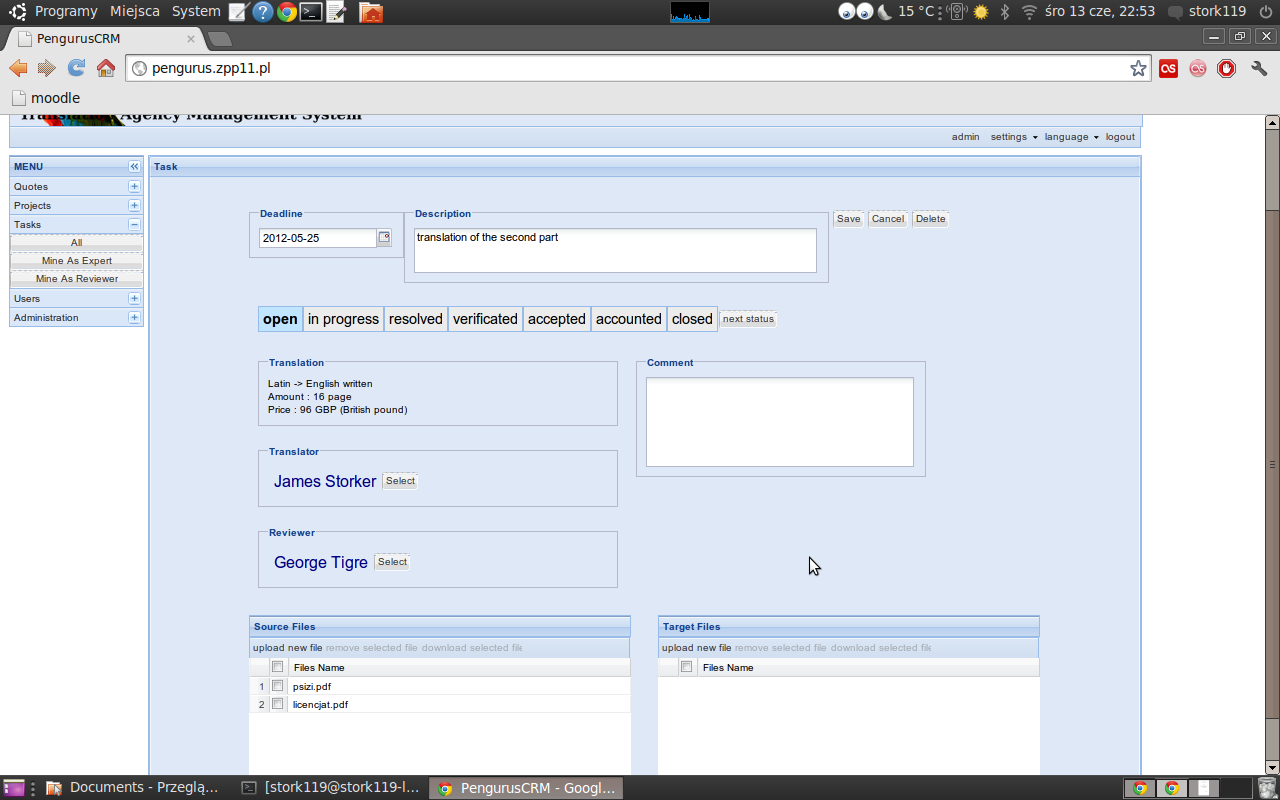
\includegraphics[width=0.8\textwidth]{resources/task.png}
\caption{Panel Zadania}
\end{figure}
\\
\item Rozliczenie - w przypadku pracowników nieetatowych, czyli tzw. freelancerów, bądź pracowników na umowę o dzieło po każdym rozwiązanym Zadaniu następuje rozliczenie. Gdy takowe zostanie wykonane księgowy zmienia status Zadania na "accounted".\\
Gdy ekspert jest pracownikiem etatowym wszystkie zadania wykonuje automatycznie Menadżer Projektu.
\item Zakończenie - Po rozliczeniu Zadania Menadżer Projektu może go zakończyć,a wszystkie pliki i informacje z nim związane trafiają do archiwum. 
\end{enumerate}


\chapter{Rozwiązania}
\section{Spring Framework}
Spring Framework jest jedną z najpopularniejszych i najlepiej działających platform programistycznych dla Javy. Zalet tego frameworku jest wiele, poniżej przedstawione zostały jednak te najbardziej zauważalne w pracy nad naszym projektem.

\paragraph{Wzorzec projektowy MVC}
Spring MVC jest jednym z pakietów oferowanych przez Spring Framework. Został on zaprojektowany do tworzenia aplikacji działających na bazie wzorca projektowego Model-View-Controller i oferuje wiele mechanizmów ułatwiających pracę z nimi. Przebieg akcji z użyciem Spring MVC w naszej aplikacji wygląda następująco:

\begin{itemize}
  \item Klient prosi o zasoby aplikację
  \item Zapytanie jest przechwytywane przez Spring Front Controller które zajmuje się znalezieniem odpowiednich mapowań adresów
  \item Mapowania wykorzystywane są do znalezienia odpowiedniego kontrolera aplikacji odpowiadającego za odpowiedzenia na zapytanie
  \item Kontroler przetwarza zapytanie i generuje lub odnajduje dane, o które poproszono w zapytaniu
  \item Przygotowane dane zostają zserializowane
  \item Wynik jest odsyłany do klienta
\end{itemize}

Dodatkową zaletą implementacji tego modelu przez Spring jest fakt, że pozwala on na integrację z innymi frameworkami i wybór obiektów odpowiedzialnych za wykonanie poszczególnych akcji, co jest jedną z większych motywacji. W projekcie bowiem wykorzystujemy to do połączenia tego modelu z możliwościami oferowanymi przez frameworki Hibernate i ExtGWT.

To właśnie dlatego w przepływie tym pominięte zostało generowanie widoku na podstawie danych, gdyż klientem jest samodzielny framework prezentujący dane użytkownikowi.

\paragraph{Inwersja kontroli}
Inwersja kontroli (ang. IoC) to w programowaniu obiektowym praktyka, w której powiązania obiektów ustalane są dopiero podczas wykonania, a nie w trakcie kompilacji. Jest to bezpośrednio związane z oddzieleniem logiki aplikacji od kodu. Główną metodą osiągnięcia tego celu jest stosowanie Dependency Injection, co oznacza, że obiekty są "wkładane" jeden w drugi.

Spośród kilku możliwych technik implementacji inwersji kontroli Spring implementuje dwie: z użyciem konstruktora oraz z użyciem setterów. W naszej aplikacji używamy tej drugiej. Do konfigurowania zależności pomiędzy obiektami używamy plików xml, w których znajdują się definicję fasolek (ang. beans) dla zarządzanych obiektów oraz ustawienia zależności między nimi.

IoC zwiększa znacząco czytelność kodu i zmniejsza jego ilość, a co ważniejsze, do minimum skraca się czas potrzebny do zarządzania tworzeniem, usuwaniem, przekazywaniem i łączeniem obiektów tworzących aplikację w spójną całość. Dodanie zależności obiektów sprowadza się stworzenia metod $set()$ and $get()$ oraz dołączenia odpowiedniego wpisu w pliku konfiguracyjnym.

Podział nieprzeplatających się ze sobą modułów implementujących określone interfejsy pozwala skupić się na ich rzeczywistym przeznaczeniu dodatkowo zwiększając testowalność kodu pozwalając na podstawianie spreparowanych obiektów w miejsce zależności.

\paragraph{Spring Security}
Jednym z projektów wchodzących z zestaw Springowych narzędzi jest Spring Security. Projekt ten implementuje pełen zestaw funkcjonalności związanych z bezpieczeństwem aplikacji począwszy od logowania (czy to z własnym systemem użytkowników, LDAPem, OAUTHem) skończywszy na filtrowaniu danych przesyłanych do użytkownika.

Pierwszym miejscem w którym wykorzystujemy tą część frameworku jest strona logowania. Osoba nieautoryzowana przez system próbująca dostać się do zasobów (w tym przypadku samej aplikacji), do których nie ma uprawnień zostaje przekierowana na stronę logowania. Osoba zalogowana, ale bez uprawnień po prostu zostanie o tym poinformowana. Spring pozwala definiować prawa dostępów do zasobów na podstawie ról użytkowników oraz adresów zasobów, co odbywa się już na poziomie dyspozytora (ang. dispatcher).

Sam mechanizm logowania jest również odpowiedzialnością Spring Security. Mechanizm ten wykorzystuje naszą własną implementację systemu użytkowników dopasowaną do odpowiedniego interfejsu. Informacja o tym jaki użytkownik jest zalogowany zostaje zapamiętana wewnątrz sesji i jest dostępna w każdym miejscu, które wymaga jej użycia. To także Spring zapewnia szyfrowanie haseł użytkowników z użyciem hashu nazwy użytkownika i soli.

Ostatecznie projekt ten wykorzystujemy do ograniczania dostępu do konkretnych funkcji oferowanych przez stronę serwera aplikacji lub danych przez nie zwracanych. Osiągamy to przy użyciu systemu adnotacji, które umieszczone przed definicją metody definiują dla niej cechy bezpieczeństwa. W ten sposób określamy, czy użytkownik może wywołać tę funkcję na podstawie jego roli, bądź przy użyciu zdefiniowanych przez siebie warunktów. W podobny sposób możemy przefiltrować kolekcję obiektów zwracanych przez funkcję. 

\section{Google Web Toolkit (ExtGWT)}
Framework do budowania aplikacji webowych w oparciu oparciu o AJAX, przy użyciu języka Java, tak w skrócie można opisać Google Web Toolkit.
zalety gwt i alternatywy (inne gwt, UiBinder)

\section{Hibernate}
Hibernate jest najpopularniejszą biblioteką mapowania obiektowo-relacyjnego przeznaczoną dla języka prograwania Java.
Zapewnia ona przede wszystkim translację danych pomiędzy relacyjną bazą danych, a światem obiektowym. 
Opiera się na wykorzystaniu opisu struktury danych za pomocą języka XML lub annotacji, dzięki czemu można mapować obiekty, 
bezpośrednio na istniejące tabele bazy danych. Cechy biblioteki: 
\begin{itemize}
\item wysoka wydajność (leniwa inicjalizacja, wiele strategii pobierania danych)
\item wiarygodność i skalowalność (używana przez dziesiątki tysięcy deweloperów)
\item rozszerzalność
\item obszerne wsparcie języków zapytań (HQL, JPAQL, SQL) 
\end{itemize}
Hibernate zawiera wiele zalet i możliwości. Poniżej zostały opisane te, które 
są najbardziej zauważalne i pomocne w naszej aplikacji.

\paragraph{Mapowanie za pomocą języka XML}
Mapowania za pomocą języka XML jest jednym z dwóch mechanizmów mapowania oferowanych przez Hibernate. Umożliwia przeniesienie 
w prosty sposób całej hierarchii klas na język bazy danych. Do każdej klasy z hierarchii należy storzyć odpowiadający jej plik XML, 
który powie Hibernate'owi jaką ma stworzyć tabele do bazy danych. W pliku tym możemy zawrzeć wiele informacji, na przykład:
\begin{itemize}
\item czy kolekcje będa leniwie wyjmowane (opcja lazy)
\item relacje między poszczególnymi klasami (wiele do wielu, jeden do wielu, itp.)
\item czy przy zapisywaniu/usuwaniu obiektu równiez obiekty, które są z nim powiązane będą zapisywane/usuwane (opcja cascade)
\item dziedziczenie występujące miedzy klasami
\end{itemize}
Nasz zespół skrócił sobie czasy pracy nad plikami XML poprzez wykorzystanie wtyczki do Eclipse'a, która automatycznie je generuje   
na podstawie zaimplementowanych klas. Często jednak należy poprawić te pliki, ponieważ wtyczka ta nie radzi sobie z odwzorowaniem 
asocjacji między klasami. Wykorzystanie mechanizmu mapowania Hibernate'a zaoszczędziło nam wielu czasu, który musielibyśmy przeznaczyć 
na planowanie struktury bazy danych.

\paragraph{Data access object}
Jest to obiekt, który zapewnia interfejs do bazy danych jednocześnie nie ujawiając jej szczegółów. Głównym celem stosowania DAO jest
oddzielenie logiki biznesowej od dostępu do danych. W naszej aplikacji został wykorzystany wzorzec generycznego DAO, który oferuje 
pięć metod: create, read, update, delete (CRUD) oraz loadAll, które odpowiednio: tworzą nowy obiekt, wyjmują obiekt, aktualizują 
istniejący obiekt, kasują obiekt oraz pobierają wszystkie obiekty danej klasy z bazy danych. Każda klasa z modelu danych ma własny 
obiekt DAO dziedziczący po tym generycznym. Rozwiązanie to zaoszczędziło nam czas, który musielibyśmy poświęcić na implementowanie 
dla każdej z osobna klasy operacji CRUD. Niektóre DAO posiadają dodatkowe, bardziej skomplikowane metody jak na przykład wyjęcie projektów, 
w których brał udział kierownik o danym identyfikatorze. Wykorzystanie DAO skutkuje stworzeniem dodatkowej warstwy interfejsu ale dzięki 
temu kod staje się czytelniejszy, ponieważ szczegóły przechowywania danych są ukryte. Operacje na bazie danych ograniczają 
się tylko do wywołania odpowiedniej metody z DAO.

\paragraph{Znajomość biblioteki} 
Ważnym czynnikiem, który pomógł nam w wyborze Hibernate'a był fakt, że trzy osoby z naszego zespołu 
były już dobrze zaznajomione z biblioteką, ponieważ w tym samym czasie uczęszczały na zajęcia z zaawansowanych baz danych, na których 
poznały podstawy działania oraz możliwości biblioteki. Zanim rozpoczęliśmy pracę na kodem naszej aplikacji te trzy osoby zdążyły już 
napisać dwa programy z wykorzystaniem Hibernate'a i wyniosły same pozytywne doświadczenia. Stwierdziliśmy, że lepiej wykorzystać narzędzie, 
które już poznaliśmy, wypróbowaliśmy i wiedzieliśmy, że jest dobre i w pełni spełnia nasze oczekiwania, niż szukać czegoś nowego.

\paragraph{Alternatywne narzędzie - TopLink}
TopLink jest taka samo jak Hibernate biblioteką mapowania obiektowo-relacyjnego dla języka programowania Java. Cechy TopLink:
\begin{itemize}
\item zestaw mapowań bezpośrednich i relacyjnych
\item mapowanie obiektów do XML
\item obsługuje wiele języków zapytań
\item wizualny edytor mapowania
\item keszowanie w celu zapewnienia tożsamości obiektu
\end{itemize}
Głównym powodem dla którego zdecydowaliśmy się na Hibernate'a, a nie na TopLink'a był fakt, że większa część zespołu miała już 
doświadczenie związane z użyciem tej pierwszej biblioteki, która całkowicie spełniała nasze wymagania związane z tworzeniem bazy 
danych. Kolejnym argumentem przeciwko TopLink był fakt, że musielibyśmy poświęcić czas na jego poznanie, który moglibyśmy 
przeznaczyć na implementacje.

\section{System klas i uprawnień użytkowników}
Projektowana przez nas aplikacja w oczywisty sposób musiała przechowywać dane użytkowników oraz umożliwiać im logowanie się do systemu. Mogliśmy podjąć jedną z dwóch decyzji: wykorzystać istniejący system w oparciu o protokół LDAP, bądź też zaprojektować i zaimplementować własny system.

\paragraph{Ligh!weigh! Directory Access Protocol}
Protokół ten jest przeznaczony do korzystania z usług katalogowych za pośrednictwem protokołu internetowego. LDAP obsługuje podstawowe operacje pozwalające na logowanie, wyszukanie wpisów katalogowych, dodawanie, usuwanie, sprawdzanie i modyfikowanie wpisów oraz kilka innych. Operacje te umożliwiają przechowywanie w systemie zarządzającym autentykacją praktycznie dowolnych danych i pozwalają na unifikację systemu logowania dla wielu współdziałających aplikacji.

Do logowania w naszej aplikacji nie użyliśmy jednak tego protokołu. Zaprojektowany przez nas, z użyciem hierarchii klas i atrybutów, model użytkownika ma obsługiwać użytkowników wielu typów i dla każdego z nich zapamiętywać dostosowane do potrzeb aplikacji informacje. Użycie protokołu LDAP wymagałoby żmudnego, nieintuicyjnego i nierozszerzalnego mapowania pól klas na strukturę wpisów katalogowych. Jako że nie projektowaliśmy systemu mającego w założeniach integrację z innymi projektami, nic nie stało na przeszkodzie zastosowaniu innego rozwiązania.

\paragraph{Własny system}
Możliwość łatwego mapowania obiektów javowych na obiekty bazodanowe przy użycia frameworku Hibernate przekonała nas do stworzenia własnego systemu zarządzania użytkownikami. Dzięki temu mogliśmy dostosować strukturę klas przechowujących wszystkie dane użytkownika do naszych potrzeb i skonfigurować tę platformę do przechowywania i zarządzania także tymi obiektami.

Zaletą tego rozwiązania oprócz prostoty implementacji i przejrzystości kodu jest także możliwość wykorzystania wszystkich zalet oferowanych przez Hibernate.

\paragraph{System klas}
Ponieważ prawie każdy użytkownik naszej aplikacji jest osobą, w pierwszej kolejności potrzebowaliśmy klasy, która będzie przechowywała dane osobowe użytkownika (class PersonalData). Obiekt ten będzie pojawiał się jako jedno z pól użytkowników naszej aplikacji.

Użytkowników naszej aplikacji podzieliliśmy na dwie grupy - klientów i pracowników. Klient indywidualny opisywany jest przez swoje dane osobowe, klient biznesowy - nazwę firmy oraz listę danych osobowych przedstawicieli tej firmy. Pracownicy również opisywani są przy użyciu swoich danych osobowych. Jedynie ich część, osoby zatrudnione w roli tłumacza, posiadają dodatkowo informację o wykonywanych przez nich tłumaczeniach.
Wszystkie te klasy tworzą hierarchię klas użytkowników rozszerzając abstraktycjną klasę użytkownika zawierającą informacje o loginie i haśle użytkownika, liście jego ról w systemie oraz ewentualnie jego dodatkowy opis.

\paragraph{System ról}
System klas użytkowników nie wyczerpuje wszystkich typów użytkowników, które miałyby być rozróżniane i obługiwane przez naszą aplikację. Ponadto nie nadaje się on do wyznaczania uprawnień użytkownika. Dlatego każdemu użytkownikowi przypisaliśmy listę ról, które pełni on w systemie. Jest to całkiem oczywisty wybór, gdyż ten sposób opisywania uprawnień użytkownika jest powszechnie stosowany i w szczególności wpasowuje się w wymagany przez Spring interfejs. Pozwala on także na filtrowanie określonych typów użytkowników w systemie np. w momencie, gdy potrzebujemy wyślietlić użytkownikowi tylko określony ich rodzaj.

\section{Środowisko pracy}

\subsection{Git}
Spośród dostępnych na rynku darmowych i popularnych systemów kontroli wersji zdecydowaliśmy się używać GITa. Na fakt dokonania takiego wyboru wpłynęły trzy rzeczy.

Pierwszym argumentem za użyciem tego właśie systemu jest fakt, że każdy z nas miał już doświadczenie w pracy z tym narzędziem, niektórzy całkiem świeże. Pozostali spotkali się z nim chociażby w czasie jednego z uczelnianych przedmiotów.
  
Drugim argumentem za wyborem tego system jest fakt, iż GIT jest działa na zasadzie rozproszonego modelu. Pozwala to na pracę bez stałego dostępu do serwera, co w pracy nieetatowej w zmiennym środowisku pracy jest ważnym argumentem do zapewnienia ciągłości pracy nad projektem.

W końcu GIT jest systemem wersji, z którym pracuje wybrany przez nas system rewizji kodu.

\subsection{Gerrit}
Gerrit to wykorzystywane przez nas narzędzie do rewizji kodu. Powstało jako narzędzie rozwjane przez Google na potrzeby Androida. Jako sprawdzone już narzędzie Open Source okazał się dobrym wyborem.\\

Narzędzie to zostało wybrane w celu podniesienia jakości tworzonego przez nas kodu. Jako niedoświadczony jeszcze zespół musieliśmy kontrolować nawzajem produkowany przez nas kod. Rewizja kodu wpływa na jakość kodu w trojaki sposób:
\begin{itemize}
\item Ogranicza liczbę błędów w kodzie wpływającym do repozytorium
\item Pozwala na bierząco kontrolować postępy prac pozostałych członków zespołu i zapewnia ciągłość w rozumieniu architektury systemu
\item Pomaga w dzieleniu się doświadczeniem w stosowaniu rozmaitych technik wewnątrz zespołu
\end{itemize}

Ostatecznie jednak rewizja kodu sprowadzała się do kontrolowania go przez lidera naszego zespołu. W teorii posiadał największe doświadczenie i miał kontrolować pracę całego zespołu, poprawiać błędy projektowe lub pomyłki oraz zwracać uwagę na dobre zwyczaje i techniki. O ile było to możliwe w początkowym stadium rozwoju projektu, o tyle kontrola przestawała być możwliwa gdy źródła aplikacji zaczęły przyrastać impulsywnie, większymi partiami, co uniemożliwiało dokładne ich sprawdzanie. \\

Oprócz ręcznej rewizji kodu Gerrit, dzięki integracji z Jenkinsem, pozwalał na automatyczne testowanie zmian przesyłanych do repozytorium, co sprowadzało się do uruchomienia zbioru przygotowanych testów na teoretycznym stanie projektu po zaakceptowaniu zmian. Zostanie to opisane w sekcji \ref{r:jenkins}.

\subsection{Jenkins}\label{r:jenkins}
Jenkins to narzędzie Open Source napisane w Javie służące do ciągłej integracji. Narzędzie to pomaga w zapewnieniu spójności projektu. Oznacza to, że w każdym momencie istnienia projektu implementowana aplikacja kompiluje się bezbłędnie, a uruchomiona działa poprawnie. Dzięki temu ogranicza się przestoje w pracy spowodowane błędami programistycznymi za które odpowiedzialność zrzucana jest na pojedynczych członków zespołu. Jest to przyczyną także dodatkowego stresu, którego można uniknąć przez wczesne wykonanie błędnego fragmentu kodu.

\paragraph{Testowanie kodu}
Jedną z dwóch odpowiedzialności zrzuconych na to narzędzie było częste wykonywanie przygotowanych wcześniej testów. W podstawowej konfiguracji możliwe jest, aby testy były wykonywane cyklicznie, co pewien czas. Jest to odpowiedni model gdy projekt ulega częstym zmianom które wymagają stałego uruchamiania testów. W naszym przypadku, to jest pracy niedoświaczonego, małego zespołu, lepszą metodą jest wykonywanie testów po każdej zmianie stanu repozytorium, a wręcz przed jej dokonaniem. Dzięki integracji z narzędziem do rewizji kodu na każdej zmianie wprowadzanej do repozytorium wymuszone zostały dwa warunki: dodany fragment kodu powinien zostać zaakceptowany przez osobę kontrolującą kod oraz musiał przechodzić zadane testy.

\paragraph{Przykładowa aplikacja}
Drugą odpowiedzialnoścą Jenkinsa było uruchamianie przykładowej wersji aplikacji. Pozwalało to na wykrywanie błędów interfejsu aplikacji w produkcyjnej jej wersji, ułatwiało projektowanie aplikacji oraz prezentowało samą aplikację zainteresowanym osobom.

Działająca w ten sposób aplikacja była dla nas wielką pomocą i ułatwieniem. Aplikacja uruchomiana lokalnie w trybie developerskim uruchamiała się bardzo długo, zużywała ogromną ilość zasobów komputera oraz działała niesamowicie wolno, przez co stawała się całkowicie nieprzydatna w celu szybkiego sprawdzenia jej stanu i wyszukiwania drobnych błędów. Dodatkowo pełna kompilacja aplikacji trwała bardzo długo (od 5 do 15 minut) i uniemożwiwiała pracę w tym czasie na komputerze. Dlatego też przykładowa wersja aplikacji była restartowana raz dziennie w środku nocy, bądź tez na życzenie developerów.  

\subsection{Jira}
Jira jest to oprogramowanie firmy Atlassian służące do zarządzania projektem oraz śledzenia błędów. 
Narzędzie to "łączy zespół z wykonywanym zadaniem".

\paragraph{Zarządzanie projektem} 
Podczas realizacji projektu wykorzystaliśmy metodykę agile'ową, która jest wspierana przez Jirę. 
Pozwoliła nam łatwo i wygodnie zarządzać projektem. W szczególności korzystaliśmy z :
\begin{itemize}
\item Wersjonowania wydań - dzięki temu mogliśmy wyznaczać kolejne terminy realizacji danych wersji 
  dało nam to możliwość kontrolowania postępu prac i w razie potrzeby szybko reagować na zastoje;
\item Tworzenia raportów - informowało nas o stanie realizacji projektu oraz o postępie prac przez poszczególnych członków zespołu;
\item Tworzenia zadań - przydzielanie poszczególnym członkom zespołu, ustawianie terminów, komentowanie, oraz przydzielanie zasobów 
umożliwia wygodną komunikację oraz szybkie odnalezienie się w projekcie i w zadaniu jakie zostało nam przydzielone do realizacji;
\item Plansz agile'owych - np. Planning Board, Task Board w przejrzysty sposób informowały nas o stanie realizacji poszczególnych zadań oraz o 
etapie prac nad daną wersją projektu, umożliwiały prostą i wygodną edycję tych danych wspierając przyjętą przez nas metodykę agile'ową
\item Dashboardów - podobnie jak w podpunktach powyżej służyły do informowania nas o stanie realizacji projektu i o pracy poszczególnych członków zespołu
\end{itemize}

\paragraph{Zintegrowanie z innymi komponentami}
Jira jest integrowalna z innymi produktami Atlassiana, a w szczególności wykorzystywanym przez nas Confluencem.
Ponadto zintegrowaliśmy Jirę z kontem pocztowym (gmail) dzięki czemu otrzymywaliśmy powiadomienia o przydzielonych zadaniach, bądź innych zmianach w projekcie.

Bardzo istotna była integracja z systemem kontroli wersji oraz z webowym narzędziem do przeglądu kodu.
Jira umożliwia integrację z najbardziej popularnymi systemami jak : GIT, SVN, CVS, Clearcase i inne.
W naszym przypadku wykorzystaliśmy GITa, a do przeglądu kodu za pomocą przeglądarki używaliśmy Gerrita. 
Dzięki systemowi znaczników (przypisaniu numeru Zadania z Jiry do commita) możliwy był szybki podgląd zmian w Gerricie za pomocą automatycznie dodawanych linków do Zadań w Jirze.
Integrowało to zmiany w kodzie z postępem prac umieszczonym w schematach Jiry.  

\paragraph{Produkty konkurencyjne}
Jednym z produktów konkurencyjnych, których wykorzystanie rozważaliśmy jest stworzony na wydziale MIM Uniwersytetu Warszawskiego JLoXiM Redmine.
Produkt ten posiada większość z funkcjonalności jakie posiada Jira. W szczególności umożliwia tworzenie zadań, przydzielanie ich do członków zespołu, 
konfiguracją uprawnień użytkowników i zarządzanie całym projektem. Analogicznie jak Jira generuje raporty oraz w przejrzysty sposób pokazuje stan 
realizacji projektu.
Postanowiliśmy, jednakże wykorzystać produkt Atlassianowy, ponieważ część członków zespołu pracowała pod tymi narzędziami, Jira była łatwiej integrowalna
 z innymi produktami oraz posiadała bardziej przejrzysty i zaawansowany interfejs użytkownika.
\subsection{Confluence}
Confluence jest narzędziem dla zespołów służącym do uproszczenia współpracy, dzielenia się wiedzą, dyskusją pomysłów.
W naszym projekcie był on wykorzystywany w szczególności podczas etapu projektowania systemu oraz przy tworzeninu dokumentacji.
Confluence zapewnia wiele wygodnych rozwiązań.
\begin{itemize}
\item Przejrzysty podział na projekty - tworzenie dynamicznych stron , podstron , dowiązań, projektowanie dashboardów.
\item Proste w obsłudze i wygodne wiki - dodawanie linków, mockapów, filmów, plików.
\item Udostępnia pluginy do tworzenia schematów i diagramów np.: Gliffy
\item Integracja z Officem  
\end{itemize}
\subsection{Maven}
Maven jest to narzędzie wspierające zarządzanie projektem. Służy ono do automatycznej budowy Javowego oprogramowania oraz do raportowania i tworzenia dokumentacji.

Budowa aplikacji jest określona w POM (Project Objected Model) - w Mavenie nosi nazwę pom.xml . 
POM przechowuje szczegóły budowy produktu, ale także  informacje o zespole programistów, zastosowanych systemach wspomagających rozwój oprogramowania.\\

Jedną z funkcjonalności Mavena jest system zarządzania zależnościami oraz tzw. przechodnimi zależnościami.
Maven posiada duże i ciągle rosnące repozytorium bibliotek. Użytkownik może sam określić wersję pobieranej biblioteki (w pliku pom.xml), bądź wykorzystać mechanizm Mavena, 
który dostosuje wersję do danego produktu. Poszczególne wtyczki, biblioteki są pobierane podczas pierwszego jej wykorzystania.  \\

Podsumowując, narzędzie to pozwala na łatwe i szybkie uruchamianie produktu w nowym środowisku. Dzięki niemu nie musimy samodzielnie zarządzać paczkami zawierającymi wykorzystywane przez nas biblioteki. Uruchomienie projektu na nowym serwerze bądź komputerze roboczym z dostępem do internetu sprowadza się do skopiowania źródeł projektu i użyciu jednej komendy tego właśnie narzędzia, które samo zadba o pobranie potrzebnych bibliotek, skompilowanie projektu z użyciem odpowiednich narzędzi i dostarczenie wyprodukowanego, gotowego do użycia, archiwum we wyspecyfikowane miejsce.
\subsection{Eclipse}

Eclipse to wybrane przez nas środowisko programistyczne, które łączy ze sobą zintegrowane środowisko programistyczne oraz rozszerzalność zapewnianą przez bibliotekę wtyczek umożliwiającą pracę praktycznie z każdym narzędziem. Praca z użyciem tego środowiska jest bardzo wygodna, ponieważ Eclipse udostępnia niezliczoną ilość skrótów klawiszowych umożliwiających niezwykle proste poruszanie się po całym projekcie. Podstawowe skróty obsługują nie tylko standardowe zarządzanie tekstem, ale zarządzanie kodem. Możliwe jest m. in. wydzielanie funkcji, globalne zmiany nazw klas, metod zmiennych, automatyczne tworzenie szkieletów obiektów, intuicyjne poruszanie się po strukturze hierarchii obiektów i wiele innych. Upraszcza to zmiany w istniejącym kodzie przez co samo tworzenie aplikacji staje się bardziej elastyczne, klasy czytelniejsze, a programiści nie boją się zaglądać i modyfikować kodu stworzonego przez poprzedników.

\paragraph{Wtyczki}
\begin{itemize}
\item \textbf{EGit - Git Team Provider} - wtyczka pozwalająca obsługiwać repozytorium Gita z poziomu Eclipse'a. Oprócz tego, że wtyczka ta umożliwia wykonywanie wszystkich poleceń, które dostępne są z poziomu konsoli, EGit zapewnia także dodatkowe funkcjonalności ułatwiające prace, takie jak zastępowanie fragmentu dowolnego pliku przez fragment tego samego pliku w historii gita czy możliowść szybkiego podglądu kto i kiedy jako ostani modyfikował wskazaną linię kodu. Wtyczka ta umożliwia także integrację z Gerritem.
\item \textbf{Maven Integration for Eclipse} - wtyczka integrująca eclipsa z Mavenem. Dzięki niej Eclipse potrafił wykrywać, które biblioteki spośród wymaganych przez projekt były zapewnione przez lokalne repozytorium Mavena oraz potrafił zarządzać pobieraniem tych, których brakowało.
\item \textbf{FindBugs Eclipse Plugin} - wtyczka pozwalające na używanie narzędzia FindBuds. Pozwala ono na drobnych i nie tylko błędów, łatwych do przeoczenia pomyłek lub naruszających dobre nawyki pisania w języku Java elementów kodu. Pozwala to na zmniejszenie ilości problemów, których w łatwy sposób można uniknąć.
\item \textbf{Eclipse JBoss Plugin} - wyczka pozwalająca na zainstalowanie narzędzi Hibernate Tools do pracy z Hibernatem, jak również JBoss Maven Hibernate Configurator do zintegrowania współpracy Mavena z Hibernatem
\end{itemize}

\paragraph{Netbeans}
Netbeans, podobnie jak Eclipse, jest zintegrowanym oferującym dużo możliwości ułatwiających zarządzanie projektem oraz wiele wtyczek. Podobnie jak Eclipse jest Open Source i używany przez duże grono programistów. Dlatego nie można powiedzieć, że wybór tego narzędzia byłby gorszy od dokonanego. Dlatego decyzję o wyróżnieniu jednego z tych dwóch narzędzi należy złożyć na barki opinii wyrażanych przez innych programistów oraz (znów) doświadczenia w jego obsłudze.


\chapter{Praca}
\section{Projektowanie systemu}
Rozpoczynając pracę nad projektowaniem systemu do zarządzania biurem tłumaczeń postawiliśmy sobie cel, aby w ramach tego tematu był on jak najbardziej funkcjonalny,
co oznaczało , że miał się wykazywać jak największą elastycznością w dziedzinie tłumaczeń (np. musiał uwzględniać możliwość dodania nowej usługi tłumaczeń). 
Wymagało to od nas dogłębnego przeanalizowania rynku. Nasz produkt musiał być odpowiedni dla małych biur prowadzących proste, krótkie tłumaczenia, jak i dla większych 
przedsiębiorstw, których projekty są znacznie obszerniejsze.\\

Pomocne okazały się już istniejące aplikacje. Przeanalizowaliśmy ich wady oraz zalety i wyciągnęliśmy z nich wnioski. Ponadto zauważyliśmy analogie pomiędzy procesem projektowania
systemu informatycznego, a procesem tłumaczenia. Przekładając nasze doświadczenie oraz zebrane wnioski przystąpiliśmy do tworzenia wstępnego szkicu projektu. 
Po jego uzgodnieniu zasięgnęliśmy informacji z oficjalnych dokumentów : "Polskiej Normy PL-EN 15038 Usługi tłumaczeniowe. Wymagania dotyczące świadczenia usług." oraz
schematu systemu zarządzania biurem tłumaczeń przygotowanej przez klienta.
Przyjęta kolejność miała wyeliminować niepotrzebny biurokratyczny formalizm, który utrudniłby pracę tłumaczom dla których ta aplikacja miała upraszczać ów proces, a nie go jeszcze utrudniać.\\

Projekt systemu składał się z dwóch równie istotnych części : schematu reprezentacji użytkowników oraz schematu przebiegu realizacji projektu.\\

Reprezentacja użytkowników oraz stworzony przez nas system ról został szczegółowo opisnay w punkcie 3.4. 
Jego realizacja była bardzo ciężka i czasochłonna, gdyż musiała uwzględniać problemy, jakie możemy napotkać z implementacją i wykorzystaniem tego systemu, 
a z drugiej strony musiała odzwierciedlać rzeczywisty stan podczas tłumaczenia.\\


\begin{figure}[h!]
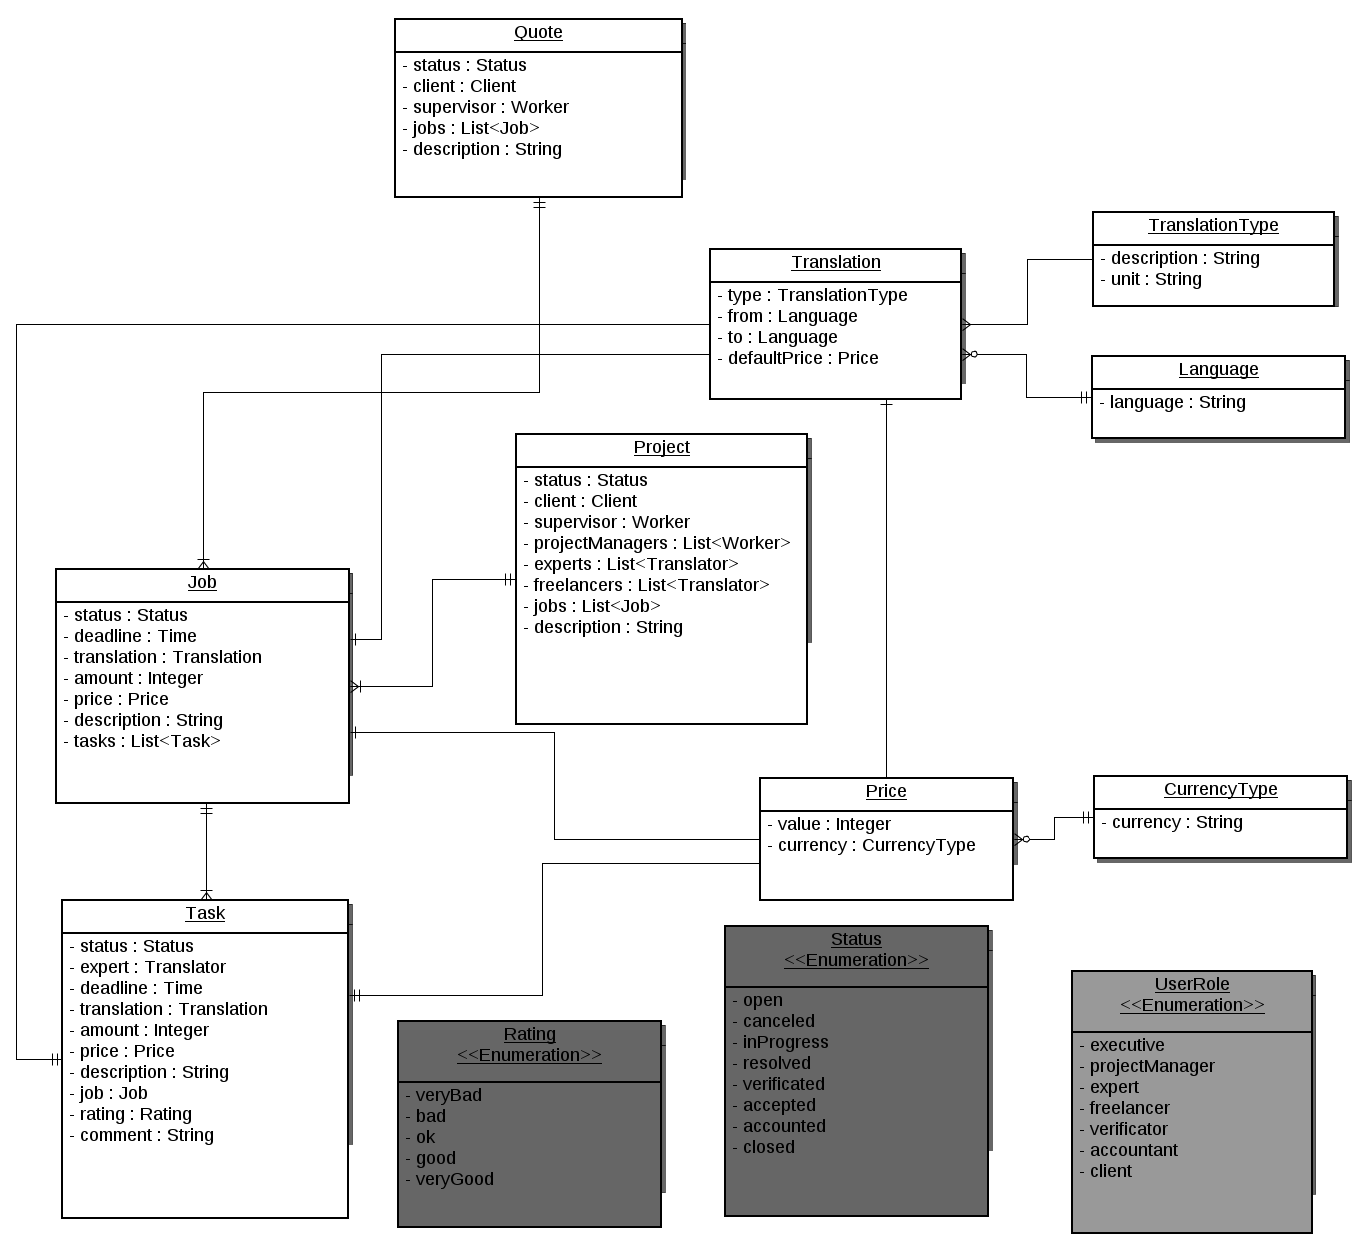
\includegraphics[width=1.1\textwidth]{resources/data.png}
\caption{Model danych zawierający wszystkie etapy przebiegu realizacji projektu}
\end{figure}


Szczegółowy opis procesu został opisany w punkcie 2. Podczas projektowania schematu rozważaliśmy różne koncepcje.
\begin{itemize}
\item Głównym problemem, jaki rozważaliśmy była ilość etapów, jakie zlecenie musi przejść od momentu rozpoczęcia do końca jego realizacji. 
Na początku schemat nie zawierał Oferty, a kontakt pomiędzy biurem tłumaczeń a Klientem miał się odbywać za pomocą Projektu. 
Postanowiliśmy, jednak dodać klasę Oferta, aby rozdzielić etap projektowania zlecenia i kontaktu z klientem od etapu realizacji - tłumaczenia. 
Służyło to poprawie przejrzystości projektu (oba etapy zawierały kompletnie różne funkcjonalności), a ponadto miało to na celu ochronę danych osobowych i własności intelektualnej.
Uważaliśmy, iż zwykli pracownicy nie powinni znać informacji o Kliencie i całym projekcie (za wyjątkiem kierowników i menadżerów),a jedynie powinni mieć dostęp do informacji zawartych w przydzielonych im Zadaniach.
 Z drugiej strony klient nie powinien znać wszystkich szczegółów realizacji projektu, a jedynie efekty poszczególnych etapów (Prac).
\item Drugim problemem z jakim się zmierzyliśmy był sposób, w jaki wyrazimy Ofertę przedstawianą Klientowi.
Chcieliśmy w prosty sposób móc przedstawić, co ma zrealizować dane zlecenie oraz podstawowe dane jakie powinno zawierać (deadline, zapłata, rodzaj tłumaczenia, dotarczone pliki).
Najprostsze rozwiązanie zakładało, iż to Oferta zawiera te informacje, co w etapie realizacji miało się prosto mapować na Projekt.
Rozważyliśmy, jednak przypadek tłumaczenia dużej książki. Klient chciałby np. aby zlecenie było realizowane etapami, bądź opłata za poszczególne części miałaby się różnić.
Przy tym rozwiązaniu należałoby stworzyć kilka Ofert, co nie byłoby wygodne. 
Postanowiliśmy zatem, aby potrakotwać zarówno Ofertę, jak i Projekt jako narzędzia, służące do zarządzania zleceniem, których poszczególne etapy (części) znajdują się w liście Prac.
To w Pracy miały zawierać się wszystkie techniczne informacje dotyczące tłumaczenia (pliki, termin realizacji, rodzaj). I tak np. na poziomie Oferty  znajdują się dane o kliencie,
możliwość wysyłania przez niego plików, a w Pracy istnieje możliwość oceny rozwiązania, jego przyjęcie/odrzucenie i zaksięgowanie.
Ponadto Praca jest współdzielona przez Ofertę jak i Projket (nie ma oddzielnych instancji).
\item Następnym problemem, jaki rozważaliśmy był nadzór nad realizacją zlecenia. Zgodnie z wymaganiami stworzyliśmy lidera tłumaczenia (u nas Menadżer Projektu), 
który zajmował się przydzielaniem Zadań do pracowników pracujących przy danym projekcie. Do projetku pracownicy byli przydzielni przez kierownika zlecenia.
Nie wiedzieliśmy natomiast ilu takich Menadżerów przypisać oraz czy powinni oni być powiązania stricte z Pracą , czy ogólniej z Projektem. 
Po długich dyskusjach i licznych pomysłach realizacji zdecydowaliśmy się na najbardziej elastyczny model. Ilość menadżerów miała zależeć od Kierownika zlecenia, który przygotował Ofertę. 
Menadżerowie mieli być przydzieleni do Projektu, tak aby nie trzeba było za każdym wybierać menadżerów do poszczególnych Prac.
Miało to byc realizowane nieformalnie.
\item Z bardziej szczegółowych problemów, jakie napotkaliśmy było stworzenie systemu typów tłumaczeń (chodziło o rozróżnienie tłumaczeń ustnych, sądowych, technicznych, itp.).
Pierwszy pomysł przewidywał stworzenie odpowiednich enumeratorów. Uniemożliwiałoby to jednak rozszerzenie - dodanie nowego rodzaju (tzn wymagałoby zmian w kodzie). 
Postanowiliśmy zatem stworzyć oddzielną klasę TranslationType posiadający odpowiednie napisy. Kierownik (admnistrator) za pomocą aplikacji mógłby dzięki temu w łatwy sposób dodać nowy typ.
\end{itemize}
Przedstawione wyżej różne problemy, na jakie natrafiliśmy podczas etapu projektowania są tylko częścią tego z czym musieliśmy się zmierzyć. 
Uważamy, że zrealizowany przez nas schemat spełnia wszystkie wymagane funkcjonalności oraz pozwala na wystarczającą zdolność przystosowania się do zmian na rynku tłumaczeń.
Ponadto liczymy na to, iż praca przy takim schemacie zapewnia wystarczającą ilość formalizmu, ale jednocześnie nie powoduje wydłużenia czasu pracy, bądź jej utrudnienia zwłaszcza w małych projektach. 

\section{Przygotowanie środowiska pracy}
Praca w zespole, w którym praca nad tymi samymi elementami projektu dzielona jest pomiędzy wiele osób wymaga stałego dostępu do wszystkich używanych narzędzi i technologii dla każdego członka zespołu. Brak takiej możliwości lub problemy z komunikacją mogą spowodować opóźnienie w pracy jednego członka zespołu, co z kolei może doprowadzić do przestoju pracy całego zespołu. Aby uniknąć takich problemów postanowiliśmy uniezależnić się od zewnętrznych dostawców sprzętu i narzędzi i stworzyć własny serwer który odpowiadałby za utrzymywanie oprogramowania do zarządzania projektem czy wykonywania testów i prezentowaniu aplikacji. \\

Zapewnienie sprzętu mającego posłużyć za bazę serwera nie stworzyło problemów, ponieważ kilku z nas posiadało w domu starszy, nieużywany sprzęt. Aby jednak serwer mógł działać sprawnie należało dokupić pamięć RAM, aby wydajnościowo mógł obsłużyć wymienione wcześniej cele. Był to jeden z kilku wydatków poświęconych temu celowi. Tak przygotowany komputer musiał spocząć w mieszkaniu jednego z nas i być stale włączony. Generowało to dodatkowe koszty. Postanowiliśmy więc podzielić wydatki pomiędzy dwa zespoły. Ponieważ wykorzystywane narzędzia mogły być używane do obsługi więcej niż jednego projektu mogliśmy zaoszczędzić pieniądze nie obciążając znacząco dodatkowo serwera. \\

Mając serwer gotowy do użycia należało zapewnić wybranym osobom z obu zespołów dostęp do niego z prawami administratora oraz wspólnie skonfigurować wybrane narzędzia. Ponieważ większość z nas do tej pory jedynie pracowała z użyciem tych narzędzi więc przygotowanie każdego z nich do pracy zabierało dużo czasu. Ponieważ niektóre z tych narzędzie miały pracować wspólnie należało poświęcić dodatkowy czas na ich integrację, a nieraz na ponowne ich instalowanie. Należy dodać, że w tej fazie rozważaliśmy jeszcze wybór dodatkowych, płatnych narzędzi, które należało wcześniej przetestować, a więc i zainstalować i skonfigurować. Ze względy na zużycie czasu na ostateczny wybór użytych narzędzi wpływał nie tylko zalety wynikające z ich eksploatacji, ale także łatwość konfiguracji i dostosowywania do potrzeb. \\

Ostatecznie w ramach przygotowania serwera do pracy zainstalowaliśmy / skonfigurowaliśmy: repozytorium (git), narzędzie do rewizji kodu (gerrit), które oczywiście kooperowało z użytym repozytorium, narzędzie do ciągłej integracji użyte do testowania i uruchamiania pokazowej wersji aplikacji (Jenkins) które odbierało polecenia od tego poprzedniego, serwer aplikacji javowych (Jetty) na których uruchamiana była aplikacja, narzędzie do zarządzania dokumentacją (Confluencem) oraz narzędzie do zarządzania projektem (Jira) zintegrowane z większością do tej pory wymienionych narzędzi. W celach administracyjnych skonfigurowane były zdalny dostęp do urządzenia (ssh), usługa udostępniająca dostęp do tych narzędzi (Apache) i narzędzie nadzorujące pracę ich wszystkich (Nagios).

\section{Problemy z użytymi narzędziami}
\subsection{Spring + ExtGWT}
Pierwszym krokiem od którego musielismy zacząć implementację aplikacji było zintegrowanie wykorzystywanych przez nas technologii. Z trzech podstawowych (ExtGWT, Spring, Hibernate) nie mieliśmy jeszcze doświadczeń z Google Web Toolkit i to w pierwszej kolejności nim należało się zająć.

W aplikacjach GWT podział struktury obiektów pomiędzy te tłumaczone na kod javascriptowy i te kompilowane i uruchamiane na wirtualnej maszynie javy wygląda następująco:

\begin{figure}[h!]
\centering
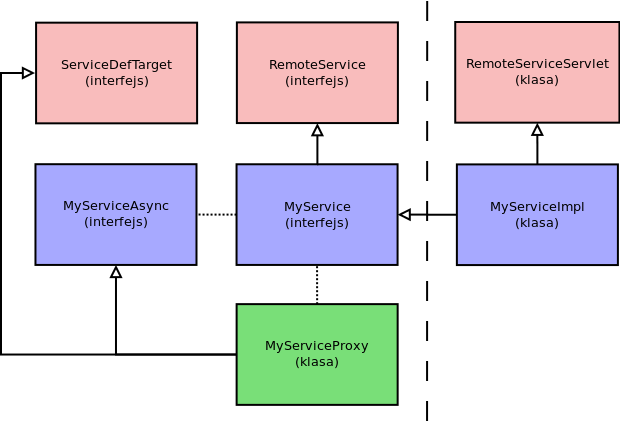
\includegraphics[width=0.60\textwidth]{resources/gwt_spring_1.png}
\caption{czerwony - importowane klasy GWT, niebieski - własne klasy, zielony - klasy generowane automatycznie}
\end{figure}

W ramach implementacji serwisów będących kolejkami RPC klasy, których metody mają być udostępniane, powinny rozszerzać importowaną z frameworku GWT klasę \textit{RemoteServiceServlet}. W ten sposób odpowiedzialność za serializowanie przesyłanych danych przekazywana jest do metod nadklasy. Dodatkowo, serwer aplikacji powinien udostępniać interfejsy implementowanych przez siebie serwisów i odpowiadające im interfejsy asynchroniczne. One, przetłumaczone do kodu javascriptowego, pozwalają klienckiej stronie aplikacji na generowanie zapytań ajax i komunikację z serwerem.

System komunikacji oparty o SOAP implementowany jest także przez platformę Spring i w naszej aplikacji to właśnie jego chcielibyśmy użyć u podstaw projektu. Klasy mające udostępniać metody serwisów muszą tutaj implementować Springowy interfejs \textit{Controller}. 

Aby uniknąć komplikacji związanych z duplikowaniem metod dla rozszerzania klasy GWT i interfejsu Springowego do rozwiązania problemu wykorzystujemy mechanizm inwersji kontroli Springa. Pomysł polega na stworzeniu klasy, która będzie tłumaczyć wywołania metod GWT na wywołania metod używanych przez platformę Spring. Do tej klasy będziemy następnie "wstrzykiwać" gotowe implementacje serwisów w jednej technologii, aby użyte mogły zostać do obsługi zapytań w drugiej.

\begin{figure}[h!]
\centering
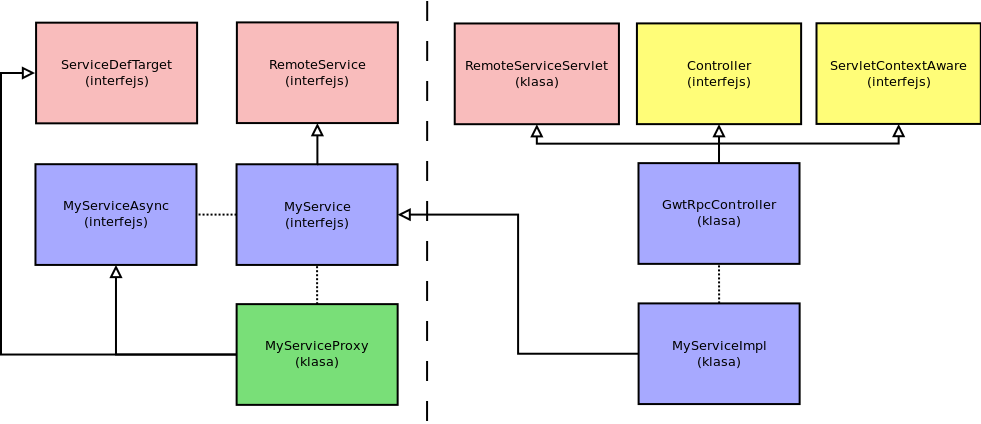
\includegraphics[width=\textwidth]{resources/gwt_spring_2.png}
\caption{czerwony - importowane klasy GWT, żółty - importowane klasy Spring, niebieski - własne klasy, zielony - klasy wygenerowane automatycznie}
\end{figure}

W naszym przypadku klasą tą jest \textit{GwtRpcController}: 
\begin{verbatim}
public class GwtRpcController extends RemoteServiceServlet implements
    Controller, ServletContextAware {
  private static final long serialVersionUID = -3618261744853211777L;
          
  private ServletContext servletContext;
  private RemoteService remoteService;
  ...
\end{verbatim}
Meteody zaimplementowane w dalszej części klasy służą do pośredniczenia pomiędzy wywołaniami metod udostępnianych przez interfejsy, a dostępem do opakowywanego obiektu. W ten sposób stworzenie nowego serwisu nie wiąże się już z duplikowaniem kodu. Aby dodać nowy serwis do tych już istniejących wystarczy implementować symboliczny jedynie interfejs RemoteService oraz dodać krótki wpis w pliku konfiguracyjnym Springa \textit{gwt-wrapper-beans.xml}. W ten sposób Spring automatycznie opakuje nasz serwis w powyższą klasę, która zadba o serializację obiektów wymaganą przez ExtGWT. 

\subsection{Hibernate}
Problemy związane z Hibernate'm wynikały głównie z powodu dużej hierarchii klas, w której występowało wiele zależności pomiędzy poszczególnymi klasami. 
Najwięcej kłopotów sprawiły nam rzeczy wymienione poniżej:
\begin{itemize}
\item odwzorowanie asocjacji pomiędzy klasami,
\item leniwe wyjmowanie kolekcji.
\end{itemize}
\textbf{Odwzorowanie asocjacji pomiędzy klasami.}

Pierwszym problem na jaki natrafiliśmy podczas implementowania bazy danych było odwzorowanie asocjacji pomiędzy klasami tak jak to było zaplanowane 
w modelu danych. Pliki z mapowaniami wygenerowaliśmy za pomocą wtyczki zainstalowanej w Eclipsie. Niestety mapowania te nie spełniały całkowicie 
naszych oczekiwań i musieliśmy wprowadzić odpowiednie zmiany. Na bieżąco dokonywaliśmy poprawek w mapowaniu jednocześnie sprawdzając czy wszystkie 
zmienione przez nas elementy dodają się w odpowiedni sposób do bazy danych. Była to praca bardzo żmudna, ponieważ należało przerobić i sprawdzić wiele 
klas. W celu ułatwienia sobie zadania podzieliliśmy klasy na niezależne grupy i staraliśmy się z osobna skonfigurować każdą z nich, gdy już to zrobiliśmy 
wzieliśmy się za integracje ze sobą wszystkich grup. W między czasie pisaliśmy odpowiednie testy, w których staraliśmy się pokryć wszystkie możliwe 
przypadki, jednocześnie wykrywając i naprawiając pojawiające się błędy. Zbiór testów powstał dla klażdej klasy mapowanej do bazy danych.\\\\
\textbf{Leniwe wyjmowanie kolekcji.}

W naszym systemie unikaliśmy sytuacji, w których pobierane są dodatkowe informacje związane z wyjmowanym obiektem z bazy danych, które nie są potrzebne 
w danym momencie. Dla przykładu jak chcemy wyświetlić listę wszystkich projektów, to nie potrzebujemy pobierać dla żadnego 
z projektów listy tłumaczów biorących w nim udział. W celu uniknięcia takiej sytuacji wykorzystaliśmy mechanizm oferowany przez Hibernate'a jakim 
jest leniwe wyjmowanie kolekcji. W dalszej części implementacji naszego systemu napotkaliśmy problemy z nim związane, 
ponieważ przepisując obiekty danej klasy na Data Transfer Object (opisane poniżej), staraliśmy się również przepisać jego kolekcje, do których nie 
mieliśmy dostępu. W związku z zaistniałą sytuacją musieliśmy dopisać odpowiednie metody, które wyjmowały obiekty z bazy danych wraz z wymaganymi 
kolekcjami.


\subsection{Data Transfer Object}
W pewnym momencie pracy nad implementacją naszej aplikacji doszliśmy do miejsca, w którym chcieliśmy zapewnić komunikacje pomiędzy stroną
serwera i klienta. Ponieważ korzystaliśmy z GWT, komunikację tę miał zapewnić mechanizm kolejek RPC polegającym na wywołaniu kodu 
strony serwera, który nazywany jest serwisem, przez klienta. Korzystając z doświadczenia części członków zespołu wiedzieliśmy, że 
obiekty wysyłane za pomocą kolejek RPC muszą być serializowane, to znaczy, że klasa opisująca dany obiekt musi implementować interfejs 
\textit{Serializable} lub interfejs \textit{IsSerializable}. Wobec tego wybraliśmy jedną z zamapowanych do bazy danych klas, która implementowała jeden z 
dwóch wyżej wymienionych interfejsów, napisaliśmy dla niej odpowiedni serwis i test, który miał pobrać obiekt z bazy danych, wysłać go na stronę klienta
i wyświetlić informacje, które ze sobą ten obiekt niesie. Niestety test się nie powiódł, patrząc na konsole trybu developement GWT dowiedziliśmy 
się, że typ: \textit{'org.hibernate.collection.PersistentSet'}, który był zawarty w wysłanym przez nas obiekcie, nie jest serializowany. Wynik testu nas 
zaskoczył, ponieważ klasa którą chcieliśmy przesłać była serializowana i nie zawierała żadnego typu \textit{'org.hibernate.collection.PersistentSet'}.
Wobec tego zaczeliśmy szukać błędu, który zwróciła konsola GWT, w sieci. Okazało się, że obiekty wyciągane przez Hibernate'a z bazy danych są 
rozszerzone w taki sposób, żeby były trwałe. Ta trwałość nie jest osiągana bez pewnego rodzaju oprzyrządowania obiektu. W przypadku Hibernate'a 
biblioteka \textit{Javassist} faktycznie zastępuje i przepisuje kod bajtowy tych obiektów przez trwałe encje. Dla kolejek RPC ma to takie 
znaczenie, że do czasu kiedy obiekt jest gotowy do przesłania nie jest tym samym obiektem, który kompilator myslał, 
że będzie wysyłany, więc podczas próby deserializacji, mechanizm GWT RPC nie wie dłużej jaki jest typ i odmawia deserializowania go.
Bogatsi o nową wiedzę zaczeliśmy szukać rozwiązania trapiącego nas problemu, niestety przez dłuższy czas nie byliśmy w stanie znaleźć żadnego 
rozwiązania i do zespołu wkradło się pewne zawahanie czy na pewno dobrze zrobiliśmy probując łączyć ze sobą GWT i Hibernate. 

Na szczęście nie poddaliśmy się i jednemu z nas udało się znaleźć rozwiązanie naszego kłopotu. Remedium okazał się wzorzec projektowy Data Transfer Object (DTO).
DTO jest prostym Plain Old Java Object, zawierającym jedynie te pola, do których możemy mieć dostęp po stronie klienta w celu wyświetlenia ich 
na stronie. Obiekt Hibernate'owy może być stworzony za pomocą danych zawartych w DTO co umożliwia przesłanie danych ze strony klienta i zapisanie ich 
w bazie danych, tak samo można stworzyć DTO korzystając z informacji zawartych w obiektach Hibernate'owych, ale wówczas już nie są przepisywane typy, które 
nie umożliwiały przesyłanie danych z serwera do klienta. Tak stworzony obiekt gotowy jest do przesłania za pomocą kolejki RPC. Oczywiście DTO również musi być 
serializowany.

Wykorzystanie wzorca projektowego DTO wiązało się z dodatkową pracą, ponieważ każda klasa z modelu danych musiała być na nowo napisana jako DTO. Dodatkowo 
trzeba było dopisać metody, które kopiowałyby obiekty Hibernate'owe z bazy danych do ich odpowiedników DTO oraz metody, które na podstawie DTO tworzyłyby obiekt 
Hibernate'owy gotowy do zapisu do bazy danych. Ponadto trzeba było zwracać uwagę na opcje leniwego wyciągania elementów z bazy danych i w zależności od nich 
wykorzystać odpowiednią technika przepisywania obiektów.

Wydaje nam się, że wykorzystanie wzorca projektowego Data Transfer Object okazało się dobrym ruchem, ponieważ dzięki niemu mogliśmy zacząć przesyłanie lekkich 
obiektów między serwerem i klientem oraz zmusiło nas to do myślenia nad strategiami kopiowania obiektów jako, że wyciagając z bazy danych pełny graf 
obiektu Hibernate'owego optymalizujemy go pod kątem tego, co jest potrzebne do wyświetlenia na stronie.

% te dwa podpunkty można ując inaczej
\section{Zasoby czasowe i organizacja pracy}
Kiedy mowa o realizacji projektu, należy zwrócić uwagę na nakład i styl pracy z nim związany. 
Poddajmy analizie przebieg realizacji projektu Pengurus CRM w kontekście zasobów czasowych oraz przyjętego schematu pracy.\\

Realizacja projektu była rozłożona na niemal jeden pełny rok akademicki i w naturalny sposób podzieliła się na dwa etapy. 
Pierwszy etap można uznać za część teoretyczną, która opiewała w przygotowanie różnej maści dokumentów stanowiących fundament do implementacji projektu, 
m.in. wizja, model danych, mapa aplikacji.
W trakcie trwania tego etapu rodziły się wszelkie pomysły, które wykrystalizowały ostateczny obraz projektu. 
Już w trakcie pierwszego miesiąca zespół zdał sobie sprawę, że pogodzenie regularnych zajęć, wymagających bieżącej nauki
(kolokwia, zadania zaliczeniowe, etc.) z pracą nad projektem licencjackim nie będzie prostym zadaniem. 
Wizja spotkań trzy razy w tygodniu, szybko została zredukowana do kilkugodzinnych spotkań raz w tygodniu, 
w trakcie których rozwiązywano bieżące problemy i rozdzielano zadania na najbliższy tydzień. 
Taki cykl pracy przyświecał niemal przez cały pierwszy etap realizacji projektu.
Przygotowanie każdego z dokumentów poprzedzone było debatą, 
a następnie do przygotowania ostatecznej formy dokumentu delegowane były dwie osoby z zespołu.\\

Taki styl pracy uległ drastycznej zmianie kiedy wkroczyliśmy w drugi etap projektu, czyli implementację.
Plan pracy stał się nieregularny i całkowicie zależny od innych obowiązków związanych głównie z uczelnią, 
największy wpływ miała z pewnością sesja zimowa, która ograniczyła pracę nad projektem do minimum na czas około dwóch miesięcy.
Mimo problemów i napiętego planu, drużyna starała się spotykać raz w tygodniu, aby wspólnie poświęcić czas na implementację 
kolejnych komponentów systemu. Ostatecznie jednak, największy nakład pracy nad projektem skupił sie w dwóch, około 10-cio dniowych odcinkach czasowych:
ferie zimowe oraz długi weekend majowy, kiedy to pozostałe obowiązki naukowe drużyny zostały tymczasowo odłożone na bok.\\

Pomimo pewnego rodzaju perturbacji, które pojawiały się w trakcie implementacji systemu, drużyna jednogłośnie stwierdziła,
że pomimo skokowego nakładu pracy, chwilami siegającego bardzo wysokiego poziomu, byliśmy dobrze zorganizowaną grupą.
Dzięku temu wersja RC naszego projektu pojawiła się już 23 maja 2012. 

\section{Komunikacja w zespole}
Jak każda praca zespołowa, tak i praca nad projektem Pengurus nie obyła się bez licznych dyskusji dotyczących, np. stosowanych rozwiązań, czy przydziału zadań.
Można by rzec, że chwilami dyskusje te przeradzały się w kłótnie czy małe konflikty, które wywoływały srogą ciszę w trakcie wspólnej pracy. 
Niemniej jednak, z perspektywy czasu można ocenić, że
emocje towarzyszące naszej pracy, napędzały spiralę pracy i sprawiały, że coś się działo. Nie było obojętności i monotonii, ponieważ każdy chciał udowodnić 
swoje racje. Dzięki temu wkład pracy każdego z członków zespołu stał na naprawdę wysokim poziomie.\\

Będąc przy poziomie, wiadomym jest, że każdy programista ma swoje mocne i słabsze strony. Jednych interesuje frontend, innych zarządzanie bazą danych. 
Podobna sytuacja miała miejsce wśród członków zesopłu Pengurus. Szczególnie w trakcie etapu implementacji lider zespołu starał się dobierać zadania do 
wykonawców w taki sposób, aby zgrywały się one z jego najmocniejszymi stronami. Oczywiście nie zawsze było to wykonalne, 
ale bezproblemowo w takich sytuacjach można było liczyć na pomoc partnerów. Szczególne zasługi w tej kwestii należą do lidera projektu, który swoją wiedzą 
starał się wspierać cały zespół.

\section{Widoki na przyszłość}
Po zamknięciu pewnego etapu, zawsze warto przeanalizować coś co właśnie się zakończyło. Odpowiedzmy na pytanie: Co pozostało po zamknięciu projektu Pengurus?
Czy możemy mówić o sukcesie? Wydaje się, że choć nie jest to sukces komercyjny, a zespół nie został okrzyknięty twórcą innowacyjnego oprogramowania, 
które może wprowadzić ogromne zmiany w świecie biur tłumaczeń, to osiągnęliśmy pewien sukces. Sukces, który można rozpatrywać 
w dwóch kategoriach: sukces jako zespół i osobisty sukces każdego z nas. \\

Każdy z członków zespołu spotykał się z pełym przebiegiem tworzenia aplikacji, począwszy od pomysłu, udokumentowania projektu, aż po ostatnie linie kodu 
podczas implementacji i zamknięcie projektu. Zasmakowaliśmy sukcesów i porażek, borykaliśmy się z problemami, które wspólnie rozwiązywaliśmy. Z pewnością 
jest to doświadczenie, które nie pójdzie na marne, a jedynie może się nam przydać w przyszłości. Być może jeszcze czeka nas Wspólna praca w tym samym składzie,
nikt tego nie wyklucza, w końcu aplikacja, która powstała ma w sobie pewien potencjał. Już teraz jest ona w stanie, 
który pozwala na wdrożenie do użycia w biurze, co jest właśnie objawem sukcesu grupowego. Ponadto, w przypadku dodatkowej współpracy ze specjalistami, 
można stworzyć moduł generowania dokumentów czy rozwijać moduły, które już istnieją, ale z pewnością mogą zostać ulepszone, 
zwiększając jakość i wydajność naszego systemu. \\

Gdyby jednak środowisko biur tłumaczeń nie okazało się dobrym celem, z narzędziami, które poznaliśmy i pomysłami jakie mamy po realizacji projektu Pengurus, 
z pewnością moglibyśmy podjąć się stworzenia systemu do zarządzania innym biurem. Bądź też, nie ograniczając się do jednej grupy odbiorców, 
systemu na tyle generycznego, że potrafiłby się dostosować do obługi szerokiej gamy biur. 
Możliwości jest wiele, a to czy jakaś z nich wejdzie w życie z pewnością pokaże czas.

\chapter{Podział pracy w zespole}
Tytułem zakończenia, należy przejść do omówienia wkładu pracy poszczególnych członków zespołu w realizację projektu Pengurus.

Będziemy bazować na wspomnianym wcześniej podziale pracy na dwa etapy: przygotowywanie dokumentacji i implementacja systemu.
\section{przygotowanie dokumentacji}
Ten etap pracy rozłożył się między członków grupy niemal równo. Wszelkie ustalenia i pomysły przedstawiane były na wspólnych spotkaniach,
natomiast spisywanie dokumentów, bądź też przygotowywane było w parach. Dla przykładu: w trakcie proseminarium, prezentację narzędzi jakich planujemy użyć
przeprowadzili wspólnie Karol Nienałtowski oraz Jakub Oćwieja, natomiast przedstawienie technologii przy użyciu których będziemy realizować projekt, przypadło parze: Michał Sabaciński i Krzysztof Gogolewski.

\section{implementacja systemu}
W odróżnieniu od wcześniejszego etapu, implementacja systemu składała się z wyraźnie odrębnych elementów, których realizacjami zajmowali
się poszczególni członkowie. Najłatwiejszą metodą omówienia wkładu pracy poszczególnych członków grupy,
będzie zaprezentowanie tych elementów i wskazanie osób, które nad nimi pracowały. W miarę możliwości postaramy się także wskazać,
co dokładnie dana osoba zrealizowała w omawianej części implementacji systemu.

\paragraph{baza danych}
Implementacja klas występujących w systemie, które będą przechowywane w bazie danych oraz dokonanie mapowania obiektowo-relacyjnego 
spoczywało w rękach Michała Sabacińskiego oraz Krzysztofa Gogolewskiego. Głównym ich zadaniem była realizacja takiego mapowania,
które gwarantuje, że przyszłe zapytania do bazy danych będą wyciągać tylko potrzebne informacje, np. obiekt nie zwraca wszystkich
swoich kolekcji kiedy nie jest to potrzebne (mechanizm leniwego wyliczania w hibernate). Następnym ich zadaniem było zaimplementowanie 
obiektów DAO, do komunikacji z bazą danych, po jego realizacji dokonaliśmy podziału. Michał zajął się pisaniem testów do bazy i obiektów DAO, 
natomiast Krzysztof dopisywał funkcje, które były potrzebne osobom piszącym już wyższą warstwę projektu, tzn. realizowali funkcjonalności.

\paragraph{bezpieczeństwo}
Realizacją bezpieczeństwa aplikacji zajął się Jakub Oćwieja. Zapewnił on bezpieczne logowanie, w oparciu o możliwości jakie daje Spring oraz
zapewnił obustronne filtrowanie danych, zarówno po stronie klienta jak i serwera, aby nie dopuścić do przekazania bądź wyświetlenia danych
użytkownikowi, który nie jest do tego uprawniony. Skoro natomiast jesteśmy już przy użytkownikach, należało zaimplementować hierarchię użytkowników, 
omówioną we wcześniszych rozdziałach tej pracy. Powstanie tej hierarchii to także zasługa Jakuba, 
jej sprawna realizacja pozwoliła na efektywne zarządzanie użytkownikami systemu i zapewniła wysokie bezpieczeństwo aplikacji.

\paragraph{funkcjonalności dot. procesu tłumaczenia}
Główną osobą i w zasadzie patronem tego etapu implementacyjnego był Karol Nienałtowski. Przygotował on silnie generyczną hierarchię klas składającą
się na realizacje procesu tłmuaczenia, od stworzenia zlecenia, aż do zamnięcia projektu tłumaczeniowego. Dzięki starannie przygotowanej hierarchii
oraz wymodelowaniu efektywnego dziedziczenia, przebieg tłumaczenia bardzo dobrze realizuje założenia normy do której nasz system miał być dostosowany.
W momencie, kiedy praca nad bazą danych w zasadzie dobiegła końca, pomocnicze funkcjonalności i klasy implementował Krzysztof.

\paragraph{funkcjonalności dot. administracji systemu}
Zarządzanie językami translacji, walutami dostępnymi przy realizacji płatności, tworzeniem obiektów translacji dla tłumaczy oraz innymi funkcjonalnościami
związanymi z administracyjną częścią systemu zajmował się Michał. Swoją część w tym rozdziale implementacji miał także Jakub, który zapewnił tworzenie użytkowników,
które w zasadzie powstawało już na etapie realizacji bezpieczeństwa systemu.

\paragraph{zarządzanie plikami}
Przetrzymywanie plików zgłoszonych do tłumaczenia, jak i plików już przetłumaczonych to zasługa Michała i Jakuba. Przygotowali oni mechanizm, który pozwalał
zarządzać plikami zarówno po stronie klienta jak i serwera.

\paragraph{front-end}
Końcowa faza projektu, to nadanie w miarę przyjaznego, intuicyjnego dla użytkownika interfejsu aplikacji. Tą częścią implementacji zajmował się Krzysztof,
korzystając z możliwości proponowanych przez GWT starał się nadać systemowi wygląd, który zachęca do użytkowania.

\paragraph{pozostałe}
Oczwiście nie wszystko co zostało wykonane w projekcie podlega klasyfikacji do powyższych kategorii. Poniżej znajdują się te części pracy, 
które nie znalazły swojego miejsca.
\begin{itemize}
\item wdrożenie mechanizmu internacjonalizacji oraz dokonanie tłumaczenia aplikacji to zasługa Karola i Michała,
\item stworzenie mechanizmu stronicowania, do porcjowania przesyłanych danych między klientem i serwerem, przygotował Jakub,
\item przygotowanie loga systemu i plakatu prezentującego projekt zawdzięczamy Jakubowi i Krzysztofowi.
\end{itemize}

\chapter{Załączone pliki}

\begin{itemize}

\item \textit{/readme} - instrukcja zawierająca opis uruchomienia aplikacji
\item \textit{/sources}
\begin{itemize}
	\item \textit{/PengurusCRM} - folder zawierający źródła projektu będące przygotowanymi projektami Eclipse'owym, Mavenowym i GWT.
\end{itemize}
\item \textit{/documents} - folder zawierający treść pracy licencjackiej i jej źródła
\item \textit{/libraries}
\begin{itemize}
	\item \textit{gxt-2.2.5-gwt22.jar} - biblioteka niezbędna do zbudowania aplikacji ze źródeł
	\item \textit{PengurusCRM.war} - paczka z aplikacją gotowa do uruchomienia z użyciem dowolnego kontenera javax.servlet
\end{itemize}
\item \textit{/additional}
\begin{itemize}
	\item \textit{/pengurus-prezi} - folder zawierający prezentację licencjacką stworząną z użyciem aplikacji Prezi
	\item \textit{/videos} - folder zawierający nagrania użyte podczas prezentacji licencjackiej
\end{itemize}
\end{itemize}

\chapter{Bibliografia}

\begin{itemize}
\item Podręcznik Spring Framework w wersji 3.1 \\
\url{h!tp://static.springsource.org/spring/docs/3.1.x/spring-framework-reference/h!ml/}
\item Tutorial Google Web Toolkit \\
\url{h!tps://developers.google.com/web-toolkit/doc/latest/tutorial/}
\item Biblioteka komponentów ExtGWT \\
\url{h!tp://www.sencha.com/examples/}
\item Podręcznik frameworku Hibernate w wersji 3.6 \\
\url{h!tp://docs.jboss.org/hibernate/orm/3.6/reference/en-US/h!ml/}
\item Przewodnik użytkownika EGit \\
\url{h!tp://wiki.eclipse.org/EGit/User_Guide/}
\item Dokumentacja Jiry \\
\url{h!tps://confluence.atlassian.com/display/JIRA/}
\item Dokumentacja Confluence'a \\
\url{h!tps://confluence.atlassian.com/display/DOC/}

\end{itemize}

\begin{comment}

\chapter*{Wprowadzenie}
\addcontentsline{toc}{chapter}{Wprowadzenie}

Blabalizator ró¿nicowy jest podstawowym narzêdziem blabalii
fetorycznej.  Dlatego naukowcy z~ca³ego ¶wiata prze¶cigaj± siê
w~próbach efektywnej implementacji.  Opracowana przez prof. Fifaka
teoria fetorów $\sigma$-$\rho$ otwiera w~tej dziedzinie nowe
mo¿liwo¶ci.  Wykorzystujemy je w~niniejszej pracy.

Przystêpne wprowadzenie do blabalii fetorycznej mo¿na znale¼æ w~pracy
Fifaka i~Gryzogrzechotalskiego \cite{ffgg}.  Dlatego w~niniejszym
tek¶cie ograniczymy siê do przypomnienia pojêæ podstawowych.

Praca sk³ada siê z~piêciu rozdzia³ów i~dodatków.
W~rozdziale~\ref{r:pojecia} przypomniano podstawowe pojêcia blabalii
fetorycznej.  Dotychczasowe próby implementacji blablizatora
ró¿nicowego zestawiono w~rozdziale~\ref{r:losers}.
Rozdzia³~\ref{r:fifak} przedstawia teoriê Fifaka i~wyja¶nia sposób jej
wykorzystania w~implementacji blabalizatora.  W~rozdziale \ref{r:impl}
przedstawiono algorytm blabalizy i~realizuj±cy go program komputerowy.
Ostatni rozdzia³ zawiera przemy¶lenia dotycz±ce mo¿liwego wp³ywu
dostêpno¶ci efektywnej blabalizy numerycznej na rozwój blabalii
fetorycznej.  W~dodatkach umieszczono najciekawszy fragment programu,
przyk³adowe dane i~wyniki dzia³ania programu.

\chapter{Podstawowe pojêcia}\label{r:pojecia}

Pojêciem pierwotnym blabalii fetorycznej jest \emph{blaba}.
Blabali¶ci nie podaj± jego definicji, mówi±c za Ciach-Pfe t-\=am
K\^un (fooistyczny mêdrzec, XIX w. p.n.e.):
\begin{quote}
  Blaba, który jest blaba, nie jest prawdziwym blaba.

\raggedleft\slshape t³um. z~chiñskiego Robert Blarbarucki
\end{quote}

\section{Definicje}

Oto dwie definicje wprowadzaj±ce podstawowe pojêcia blabalii
fetorycznej:

\begin{defi}\label{skupienie}
  Silny, zwarty i gotowy fetor bazowy nazwiemy \emph{skupieniem}.
\end{defi}

\begin{defi}\label{fetor}
  \emph{Fetorem} nazwiemy skupienie blaba spe³niaj±ce nastêpuj±cy
  \emph{aksjomat reperkusatywno¶ci}:
  $$\forall \mathcal{X}\in Z(t)\ \exists
  \pi\subseteq\oint_{\Omega^2}\kappa\leftrigh!arrow 42$$
\end{defi}


\section{Blabalizator ró¿nicowy}

Teoretycy blabalii (zob. np. pracê~\cite{grglo}) zadowalaj± siê
niekonstruktywnym opisem natury fetorów.

Podstawowym narzêdziem blabalii empirycznej jest blabalizator
ró¿nicowy.  Przyrz±d ten pozwala w~sposób przybli¿ony uzyskaæ
wspó³czynniki rozk³adu G³ombaskiego dla fetorów bazowych
i~harmonicznych.  Praktyczne znaczenie tego procesu jest oczywiste:
korzystaj±c z~reperkusatywno¶ci pozwala on przej¶æ do przestrzeni
$\Lambda^{\nabla}$, a~tym samym znale¼æ retroizotonalne wspó³czynniki
semi-quasi-celibatu dla klatek Rozkoszy (zob.~\cite{JR}).

Klasyczne algorytmy dla blabalizatora ró¿nicowego wykorzystuj±:
\begin{enumerate}
\item dualizm falowo\dywiz korpuskularny, a w szczególno¶ci
  \begin{enumerate}
  \item korpuskularn± naturê fetorów,
  \item falow± naturê blaba,
  \item falowo\dywiz korpuskularn± naturê gryzmo³ów;
  \end{enumerate}
\item postêpuj±c± gryzmolizacjê poszczególnych dziedzin nauki, w
  szczególno¶ci badañ systemowych i rozcieñczonych;
\item dynamizm fazowy stetryczenia parajonizacyjnego;
\item wreszcie tradycyjne opozycje:
  \begin{itemize}
  \item duch --- bakteria,
  \item mieæ --- chcieæ,
  \item my¶l --- owsianka,
  \item parafina --- durszlak\footnote{Wiêcej o tym przypadku --- patrz
      prace Gryzybór\dywiz G³ombaskiego i innych teoretyków nurtu
      teoretyczno\dywiz praktycznego badañ w~Instytucie Podstawowych
      Problemów Blabalii w~Fifie.},
  \item logos --- termos%\footnote{Szpotañski}
  \end{itemize}
  z w³a¶ciwym im przedziwym dynamizmem.
\end{enumerate}

\begin{figure}[tp]
  \centering
  \framebox{\vbox to 4cm{\vfil\hbox to
      7cm{\hfil\tiny.\hfil}\vfil}}
  \caption{Artystyczna wizja blaba w~obrazie wêgierskiego artysty
    Josipa~A. Rozkoszy pt.~,,Blaba''}
\end{figure}

\chapter{Wcze¶niejsze implementacje blabalizatora
  ró¿nicowego}\label{r:losers}

\section{Podej¶cie wprost}

Najprostszym sposobem wykonania blabalizy jest si³owe przeszukanie
ca³ej przestrzeni rozwi±zañ.  Jednak, jak ³atwo wyliczyæ, rozmiar
przestrzeni rozwi±zañ ro¶nie wyk³adniczo z~liczb± fetorów bazowych.
Tak wiêc przegl±d wszystkich rozwi±zañ sprawdza siê jedynie dla bardzo
prostych przestrzeni lamblialnych.  Oznacza to, ¿e taka metoda ma
niewielkie znaczenie praktyczne --- w~typowym przypadku z~¿ycia trzeba
rozwa¿aæ przestrzenie lamblialne wymiaru rzêdu 1000.

W~literaturze mo¿na znale¼æ kilka prób opracowania heurystyk dla
problemu blabalizy (por. \cite{heu}).  Korzystaj±c z~heurystyk daje
siê z~pewnym trudem dokonaæ blabalizy w~przestrzeni o~np.~500 fetorach
bazowych.  Nale¿y jednak pamiêtaæ, ¿e heurystyka nie daje gwarancji
znalezienia najlepszego rozwi±zania.  Fifak w~pracy~\cite{ff-sr}
podaje, jak dla dowolnie zadanej funkcji oceniaj±cej skonstruowaæ
dane, dla których rozwi±zanie wygenerowane przez algorytm heurystyczny
jest dowolnie odleg³e od rzeczywistego.

\section{Metody wykorzystuj±ce teoriê G³ombaskiego}

Teoria G³ombaskiego (zob.~\cite{grglo}) dostarcza eleganckiego
narzêdzia opisu przej¶cia do przestrzeni $\Lambda^{\nabla}$.
Wystarczy mianowicie przedstawiæ fetory bazowe wyj¶ciowej przestrzeni
lamblialnej w~nieskoñczonej bazie tak zwanych wy¿szych aromatów.
(Formaln± definicjê tego pojêcia przedstawiê w~rozdziale po¶wiêconym
teorii Fifaka).  Podstawow± cech± wy¿szych aromatów jest ulotno¶æ.  To
za¶ oznacza, ¿e odpowiednio dobieraj±c wspó³czynniki przej¶cia do
przestrzeni wy¿szych aromatów mo¿na zagwarantowaæ dowoln± z~góry
zadan± dok³adno¶æ przybli¿onego rozwi±zania problemu blabalizy.

Oczywi¶cie ze wzglêdu na nieskoñczony wymiar przestrzeni wy¿szych
aromatów koszt poszukiwania wspó³czynników blabalizy jest liniowy ze
wzglêdu na wymiar wyj¶ciowej przestrzeni lamblialnej.

\section{Metody wykorzystuj±ce w³asno¶ci fetorów $\sigma$}

Najchêtniej wykorzystywan± przestrzeni± wy¿szych aromatów jest
przestrzeñ fetorów~$\sigma$.  Fetory $\sigma$ daj± szczególnie prost±
bazê podprzestrzeni wid³owej.  Wi±¿e siê to z~faktem, ¿e w~tym przypadku
fetory harmoniczne wy¿szych rzêdów s± pomijalne (rzêdu $2^{-t^3}$,
gdzie $t$ jest wymiarem wyj¶ciowej przestrzeni lamblialnej).

Niestety z~fetorami $\sigma$ wi±¿e siê te¿ przykre ograniczenie: mo¿na
wykazaæ (zob.~\cite[s. 374]{ff-sr}), ¿e dla dowolnie dobranej bazy
w~podprzestrzeni wid³owej istnieje ograniczenie dolne w~metryce sierpa
na odleg³o¶æ rzutu dok³adnego rozwi±zania problemu blabalizy na
podprzestrzeñ wid³ow±.  Poniewa¿ rzut ten stanowi najlepsze
przybli¿one rozwi±zanie, jakie mo¿na osi±gn±æ nie naruszaj±c aksjomatu
reperkusatywno¶ci, wiêc istnieje pewien nieprzekraczalny próg
dok³adno¶ci dla blabalizy wykonanej przez przej¶cie do przestrzeni
fetorów $\sigma$.  Warto¶æ retroinicjaln± tego progu nazywa siê
\textit{reziduum blabicznym}.

\chapter{Teoria fetorów $\sigma$-$\rho$}\label{r:fifak}

G³ównym odkryciem Fifaka jest, ¿e fetor suprakowariantny mo¿e
gryzmolizowaæ dowolny idea³ w~podprzestrzeni wid³owej przestrzeni
lamblialnej funkcji Rozkoszy.

Udowodnienie tego faktu wymaga³o wykorzystania twierdzeñ pochodz±cych
z~kilku niezale¿nych teorii matematycznych (zob. na przyk³ad:
\cite{russell,spyrpt,JR,beaman,hopp,srinis}).  Jednym z~filarów
dowodu jest teoria odwzorowañ owalnych Leukocyta (zob.~\cite{leuk}).

Znaczenie twierdzenia Fifaka dla problemu blabalizy polega na tym, ¿e
znaj±c retroizotonalne wspó³czynniki dla klatek Rozkoszy mo¿na
przeprowadziæ fetory bazowe na dwie nieskoñczone bazy fetorów $\sigma$
w~przestrzeni $K_7$ i~fetorów $\rho$ w~odpowiedniej
quasi-quasi-przestrzeni równoleg³ej (zob.~\cite{hopp}).  Zasadnicza
ró¿nica w~stosunku do innych metod blabalizy polega na tym, ¿e
przedstawienie to jest dok³adne.

\chapter{Dokumentacja u¿ytkowa i~opis implementacji}\label{r:impl}

Program przygotowany dla systemu operacyjnego M\$ Windows uruchamia
siê energicznym dwumlaskiem na jego ikonce w~folderze
\verb+\\FIDO\FOO\BLABA+.  Nastêpnie kolistym ruchem rêki nale¿y
naprowadziæ kursor na menu \texttt{Blabaliza} i~uaktywniæ pozycjê
\texttt{Otwórz plik}.  Po wybraniu pliku i~zatwierdzeniu wyboru
przyciskiem \texttt{OK} rozpocznie siê proces blabalizy.  Wyniki
zostan± zapisane w~pliku o~nazwie \texttt{99-1a.tx.43} w~bie¿±cym
folderze.

\chapter{Podsumowanie}

W~pracy przedstawiono pierwsz± efektywn± implementacjê blabalizatora
ró¿nicowego.  Umiejêtno¶æ wykonania blabalizy numerycznej dla danych
,,z ¿ycia'' stanowi dla blabalii fetorycznej podobny prze³om, jak dla
innych dziedzin wiedzy stanowi³o og³oszenie teorii Miko³aja Kopernika
i~Gryzybór G³ombaskiego.  Z~pewno¶ci± w~rozpocznynaj±cym siê XXI wieku
bêdziemy obserwowaæ rozkwit blabalii fetorycznej.

Trudno przewidzieæ wszystkie nowe mo¿liwo¶ci, ale te co bardziej
oczywiste mo¿na wskazaæ ju¿ teraz.  S± to:
\begin{itemize}
\item degryzmolizacja wieñców telecentrycznych,
\item realizacja zimnej reakcji lambliarnej,
\item loty celulityczne,
\item dok³adne obliczenie wieku Wszech¶wiata.
\end{itemize}

\section{Perspektywy wykorzystania w~przemy¶le}

Ze wzglêdu na znaczenie strategiczne wyników pracy ten punkt uleg³
utajnieniu.

\appendix

\chapter{G³ówna pêtla programu zapisana w~jêzyku T\=oFoo}

\begin{verbatim}
[[foo]{,}[[a3,(([(,),{[[]]}]),
  [1; [{,13},[[[11],11],231]]].
  [13;[!xz]].
  [42;[{,x},[[2],{'a'},14]]].
  [br;[XQ*10]].
 ), 2q, for, [1,]2, [..].[7]{x}],[(((,[[1{{123,},},;.112]],
        else 42;
   . 'b'.. '9', [[13141],{13414}], 11),
 [1; [[134,sigma],22]].
 [2; [[rho,-],11]].
 )[14].
 ), {1234}],]. [map [cc], 1, 22]. [rho x 1]. {22; [22]},
       dd.
 [11; sigma].
        ss.4.c.q.42.b.ll.ls.chmod.aux.rm.foo;
 [112.34; rho];
        001110101010101010101010101010101111101001@
 [22%f4].
 cq. rep. else 7;
 ]. hlt
\end{verbatim}

\chapter{Przyk³adowe dane wej¶ciowe algorytmu}

\begin{center}
  \begin{tabular}{rrr}
    $\alpha$ & $\beta$ & $\gamma_7$ \\
    901384 & 13784 & 1341\\
    68746546 & 13498& 09165\\
    918324719& 1789 & 1310 \\
    9089 & 91032874& 1873 \\
    1 & 9187 & 19032874193 \\
    90143 & 01938 & 0193284 \\
    309132 & $-1349$ & $-149089088$ \\
    0202122 & 1234132 & 918324098 \\
    11234 & $-109234$ & 1934 \\
  \end{tabular}
\end{center}

\chapter{Przyk³adowe wyniki blabalizy
    (ze~wspó³czynnikami~$\sigma$-$\rho$)}

\begin{center}
  \begin{tabular}{lrrrr}
    & Wspó³czynniki \\
    & G³ombaskiego & $\rho$ & $\sigma$ & $\sigma$-$\rho$\\
    $\gamma_{0}$ & 1,331 & 2,01 & 13,42 & 0,01 \\
    $\gamma_{1}$ & 1,331 & 113,01 & 13,42 & 0,01 \\
    $\gamma_{2}$ & 1,332 & 0,01 & 13,42 & 0,01 \\
    $\gamma_{3}$ & 1,331 & 51,01 & 13,42 & 0,01 \\
    $\gamma_{4}$ & 1,332 & 3165,01 & 13,42 & 0,01 \\
    $\gamma_{5}$ & 1,331 & 1,01 & 13,42 & 0,01 \\
    $\gamma_{6}$ & 1,330 & 0,01 & 13,42 & 0,01 \\
    $\gamma_{7}$ & 1,331 & 16435,01 & 13,42 & 0,01 \\
    $\gamma_{8}$ & 1,332 & 865336,01 & 13,42 & 0,01 \\
    $\gamma_{9}$ & 1,331 & 34,01 & 13,42 & 0,01 \\
    $\gamma_{10}$ & 1,332 & 7891432,01 & 13,42 & 0,01 \\
    $\gamma_{11}$ & 1,331 & 8913,01 & 13,42 & 0,01 \\
    $\gamma_{12}$ & 1,331 & 13,01 & 13,42 & 0,01 \\
    $\gamma_{13}$ & 1,334 & 789,01 & 13,42 & 0,01 \\
    $\gamma_{14}$ & 1,331 & 4897453,01 & 13,42 & 0,01 \\
    $\gamma_{15}$ & 1,329 & 783591,01 & 13,42 & 0,01 \\
  \end{tabular}
\end{center}

\begin{thebibliography}{99}
\addcontentsline{toc}{chapter}{Bibliografia}

\bibitem[Bea65]{beaman} Juliusz Beaman, \textit{Morbidity of the Jolly
    function}, Mathematica Absurdica, 117 (1965) 338--9.

\bibitem[Blar16]{eb1} Elizjusz Blarbarucki, \textit{O pewnych
    aspektach pewnych aspektów}, Astrolog Polski, Zeszyt 16, Warszawa
  1916.

\bibitem[Fif00]{ffgg} Filigran Fifak, Gizbert Gryzogrzechotalski,
  \textit{O blabalii fetorycznej}, Materia³y Konferencji Euroblabal
  2000.

\bibitem[Fif01]{ff-sr} Filigran Fifak, \textit{O fetorach
    $\sigma$-$\rho$}, Acta Fetorica, 2001.

\bibitem[G³omb04]{grglo} Gryzybór G³ombaski, \textit{Parazytonikacja
    blabiczna fetorów --- nowa teoria wszystkiego}, Warszawa 1904.

\bibitem[Hopp96]{hopp} Claude Hopper, \textit{On some $\Pi$-hedral
    surfaces in quasi-quasi space}, Omnius University Press, 1996.

\bibitem[Leuk00]{leuk} Lechoslav Leukocyt, \textit{Oval mappings ab ovo},
  Materia³y Bia³ostockiej Konferencji Hodowców Drobiu, 2000.

\bibitem[Rozk93]{JR} Josip A.~Rozkosza, \textit{O pewnych w³asno¶ciach
    pewnych funkcji}, Pó³nocnopomorski Dziennik Matematyczny 63491
  (1993).

\bibitem[Spy59]{spyrpt} Mrowclaw Spyrpt, \textit{A matrix is a matrix
    is a matrix}, Mat. Zburp., 91 (1959) 28--35.

\bibitem[Sri64]{srinis} Rajagopalachari Sriniswamiramanathan,
  \textit{Some expansions on the Flausgloten Theorem on locally
    congested lutches}, J. Math.  Soc., North Bombay, 13 (1964) 72--6.

\bibitem[Whi25]{russell} Alfred N. Whitehead, Bertrand Russell,
  \textit{Principia Mathematica}, Cambridge University Press, 1925.

\bibitem[Zen69]{heu} Zenon Zenon, \textit{U¿yteczne heurystyki
    w~blabalizie}, M³ody Technik, nr~11, 1969.

\end{thebibliography}

\end{comment}

\end{document}


%%% Local Variables:
%%% mode: latex
%%% TeX-master: t
%%% coding: latin-2
%%% End:
